%%%%%%%%%%%%%%%%%%%%%%%%%%%%%%%%%%%%%%%%%
% Condensed thesis version (~30-35 pages)
% Original is main.tex (76 pages) — do not modify that file.
%%%%%%%%%%%%%%%%%%%%%%%%%%%%%%%%%%%%%%%%%

\documentclass[
12pt,
oneside,
english,
singlespacing,
liststotoc,
parskip,
headsepline,
]{Thesis}

\usepackage[utf8]{inputenc}
\usepackage[T1]{fontenc}
\usepackage{mathpazo}
\usepackage[backend=bibtex,
style=numeric,
bibencoding=utf8,
]{biblatex}
\addbibresource{example.bib}
\usepackage[autostyle=true]{csquotes}
\usepackage{array}
\usepackage{amssymb}
\usepackage{amsmath}
\usepackage{amsthm}
\usepackage{booktabs}
\usepackage{multirow}

\newtheorem{proposition}{Proposition}[chapter]
\newtheorem{corollary}{Corollary}[proposition]
\theoremstyle{remark}
\newtheorem*{remark}{Remark}

\geometry{
    paper=a4paper,
    inner=20mm,
    outer=20mm,
    bindingoffset=5mm,
    top=25mm,
    bottom=20mm,
}

% ============================================================
% THESIS DETAILS
% ============================================================
\thesistitle{Missing Data Imputation using Genetic Algorithms: A Distributional Approach}
\degree{Master of Technology}

\supervisor{Dr. Gaurav Srivastava}

\newcommand{\studentonename}{Madhav Umesh Kamble}
\newcommand{\studentoneroll}{MDE2025008}

\department{Department of Information Technology}
\university{Indian Institute of Information Technology, Allahabad}
\subject{Information Technology}

\newcommand{\studentnamesformatted}{\studentonename}
\newcommand{\rollnumbersformatted}{\studentoneroll}
\newcommand{\studentnamescomma}{\studentonename}
\newcommand{\studentnamesdeclaration}{\studentonename{} (\studentoneroll)}
\newcommand{\studentsignatures}{\studentonename{} (\studentoneroll)}
\newcommand{\pronounwe}{I}
\newcommand{\pronounour}{my}

\firstauthor{\studentnamesformatted}
\enrollmentnumber{\rollnumbersformatted}

\examiner{}
\addresses{}
\keywords{}
\faculty{Faculty Name}

\AtBeginDocument{
\hypersetup{pdftitle=\ttitle}
\hypersetup{pdfkeywords=\keywordnames}
}

\begin{document}
\begin{sloppypar}

\frontmatter% Use roman page numbering style (i, ii, iii, iv...) for the pre-content pages

\pagestyle{plain} % Default to the plain heading style until the thesis style is called for the body content
%----------------------------------------------------------------------------------------
%	TITLE PAGE
%----------------------------------------------------------------------------------------

\begin{titlepage}
\begin{center}
\begin{spacing}{1.2}

{\huge \bfseries \ttitle\par}  % ← Uses thesis title from main.tex

\vspace {5mm}
\textit{A thesis submitted in partial fulfillment of the requirements\\for the award of the degree of} 

\vspace{7mm}
\textsc{\huge \MakeUppercase{\degreename}}  % ← Uses degree from main.tex

\vspace {3mm}
% Logo display - no figure environment needed on title page


\includegraphics[width=5cm]{Figures/IIITA_Logo.jpg}

\vspace{5mm}
% ************************************
\large
\begin{tabular}{r@{\hspace{1.5cm}}l}
    \textit{By:-} & \textsc{\studentnamesformatted} \\[3mm]
    \textit{Enrollment No.} & \textsc{\rollnumbersformatted} \\
\end{tabular}
\\[1cm]
% *************************************

\textit{Under the Supervision of}\\[2mm]
\textsc{\Large \supname}\\% ← Uses supervisor name from main.tex
\vspace{7mm}
\textit{to the}\\[2mm]
\textsc{\Large \deptname}\\ % ← Uses department from main.tex

\vspace{8mm}
% Hindi text commented out for pdfLaTeX compatibility
% \begin{hindi}
%     \textsc{\Large {भारतीय सूचना प्रौद्योगिकी संस्थान, इलाहाबाद}} \\
% \end{hindi}
% \vspace{3mm}
\textsc{\Large \univname} % ← Uses university from main.tex

\vspace{5mm}
\today


\end{spacing}
\end{center}
\end{titlepage}


%----------------------------------------------------------------------------------------
%	CERTIFICATE
%----------------------------------------------------------------------------------------
\checktoopen
\begin{figure}[htp]
    % \centering
    
\includegraphics[width=\textwidth,height=3cm,keepaspectratio]{Figures/IIITA_Header.png}
\end{figure}
% \string\setblankpagestyle \space
\thispagestyle{empty}
\vspace*{.06\textheight}

\begin{spacing}{1.5}
\begin{center}
    {\centering\large\bfseries CERTIFICATE \par\vspace{10pt}}
\end{center}

\noindent It is certified that the work contained in the thesis titled \enquote{\ttitle} by {\studentnamescomma} has been carried out under my supervision and that this work has not been submitted elsewhere for a degree.
% ↑ Uses title and student names from main.tex

\vspace{3.5cm}
\hfill\begin{minipage}{7.5cm}   %{0.52\linewidth}
    \begin{spacing}{1.2}
        \par
        \rule{\textwidth}{0.2pt}\\
        {\supname} \par  % ← Uses supervisor name from main.tex
        {\deptname}  \par  % ← Uses department from main.tex
        IIIT Allahabad \par
    \end{spacing}
\end{minipage}

\end{spacing}
% \end{certificate}
\cleardoublepage

%----------------------------------------------------------------------------------------
%	DECLARATION
%----------------------------------------------------------------------------------------
\checktoopen
\begin{figure}[htp]
    % \centering
    
\includegraphics[width=\textwidth,height=3cm,keepaspectratio]{Figures/IIITA_Header.png}
\end{figure}
% \string\setblankpagestyle \space
\thispagestyle{empty}
\vspace{1mm}

\begin{center}
    {\large\bfseries CANDIDATE DECLARATION}
\end{center}

\begin{spacing}{1.2}

\noindent \pronounwe, \studentnamesdeclaration, hereby certify that the thesis titled \enquote{\ttitle} has been submitted by \pronounour{} in partial fulfillment of the requirements for the Degree of \degreename{} in the \deptname{} at the \univname.
% ↑ Uses pronouns and names from main.tex - automatically adjusts for single/multiple students

\par
\noindent We acknowledge that plagiarism includes: 
\begin{enumerate} 
    \item Reproducing another person's work (fully or partially) or ideas and presenting them as our own.
    \item Copying or paraphrasing another person's work without appropriate attribution.
    \item Engaging in literary theft by reproducing a unique literary construct without crediting its source.
\end{enumerate}
\par
We affirm that due credit has been given to all original authors and sources through proper citations for words, ideas, diagrams, graphics, computer programs, experiments, results, and websites that are not our own contributions. Direct quotations have been appropriately marked, and sources have been properly referenced. Furthermore, we declare that no portion of our work is plagiarized. In the event of a plagiarism claim, we accept full responsibility for the contents of this thesis. We acknowledge that our supervisor may not be able to verify the originality of every aspect of our work.
\end{spacing}

\begin{spacing}{2.0}
% \vspace{1cm}
\noindent
\begin{minipage}[t]{0.4\textwidth}  
    \begin{flushleft} 
        Place: \rule{40mm}{0.1pt}\\
    \end{flushleft}
\end{minipage}
\hfill
\begin{minipage}[t]{0.4\textwidth}
    \begin{flushright}         
        Date: \rule{40mm}{0.1pt}\\       
    \end{flushright}
\end{minipage}
% \rule{\textwidth}{0.1pt}\\
\par
{\studentsignatures} % ← Uses student names and rolls from main.tex
\end{spacing}


        
\cleardoublepage



%----------------------------------------------------------------------------------------
%	QUOTATION PAGE
%----------------------------------------------------------------------------------------

% \vspace*{0.2\textheight}
% \begin{spacing}{1.5}
% \noindent\enquote{\itshape Thanks to my solid academic training, today I can write hundreds of words on virtually any topic without possessing a shred of information, which is how I also got a good job in industry.}\bigbreak

% \hfill {\firstauthorname}
% \end{spacing}
% \cleardoublepage


%----------------------------------------------------------------------------------------
%	ABSTRACT PAGE
%----------------------------------------------------------------------------------------

\begin{abstract}
\begin{spacing}{2}

\addchaptertocentry{\abstractname} % Add the abstract to the table of contents

We prove that distributional fidelity and pointwise accuracy are structurally orthogonal objectives in missing data imputation: no single method can simultaneously minimise both. The RMSE-minimising imputation (conditional expectation) must have strictly positive distributional distance $F_r$ by the law of total variance; conversely, any $F_r$-zero imputation must have positive RMSE unless the missing values follow the same marginal distribution as the observed data. We further show this impossibility extends to neural methods: for GAIN (Generative Adversarial Imputation Networks), no reconstruction weight $\alpha > 0$ allows joint minimisation of $F_r$ and RMSE, establishing C2 as a \emph{universal impossibility theorem} for imputation.

We validate these results through a comprehensive evaluation of MIGA (Missing data Imputation via Genetic Algorithm), which directly optimises $F_r$ --- a fitness function penalising discrepancies in means, covariances, and skewness --- against MICE, KNN, and GAIN across five UCI benchmark datasets (Iris, Wine, Glass, Haberman, Wholesale) at 30\% MAR. MIGA achieves 1.5--2.0$\times$ lower $F_r$ than MICE on low-dimensional datasets (Wilcoxon $p < 0.001$), while MICE achieves 1.4--2.1$\times$ lower RMSE on every dataset. An empirical $\alpha$-sweep for GAIN ($\alpha \in \{0, 1, 10, 100, 1000, 10000\}$, all 5 datasets) confirms the impossibility holds across all reconstruction weights, revealing three failure regimes: monotone-but-off-frontier on Iris and Wine, training instability at high $\alpha$ on Haberman, and domination by MICE on both metrics on Glass.

Four additional findings characterise the scope and limits of MIGA's advantage. First, a \emph{dimension--correlation interaction} governs MIGA's advantage: a controlled $p \times \rho$ grid shows MIGA wins for $p \leq 13$ at $\rho \leq 0.6$ but loses at $\rho = 0.9$ even for $p = 8$. Second, \emph{directional MNAR} produces a striking inversion: under top-quantile missingness on Haberman, MIGA simultaneously achieves the global minimum $F_r$ (0.810) and global maximum RMSE (0.384). Third, \emph{Adaptive Diversity Injection} (AD-MIGA) replaces the fixed 90\% injection rate with an exponential decay schedule $\alpha(g) = \exp(-\lambda g / G)$, achieving lower $F_r$ on all 3 tested datasets and converging 33 generations earlier on average. Fourth, downstream evaluation shows MIGA's distributional advantage propagates to valid statistical inference on well-conditioned datasets (40--100\% KS-test pass rate, 70--95\% bootstrap CI coverage).

The thesis delivers nine contributions: the first open-source reimplementation of MIGA; the first formal proof of $F_r$--RMSE orthogonality; the first MNAR evaluation of MIGA; the first controlled $p \times \rho$ characterisation; propensity-score-weighted IPW-$F_r$ (reduces $F_r$ by 1--38\% when $n/p \gtrsim 20$); AD-MIGA adaptive diversity injection; universal orthogonality via GAIN comparison and full $\alpha$-sweep; and near-linear parallel speedup (1.94--1.98$\times$ at Q=2) via \texttt{n\_jobs}.

\end{spacing}
\end{abstract}

%----------------------------------------------------------------------------------------
%	ACKNOWLEDGEMENTS
%----------------------------------------------------------------------------------------

\begin{acknowledgements}
\begin{spacing}{1.5}
\addchaptertocentry{\acknowledgementname} % Add the acknowledgements to the table of contents

I would like to express my sincere gratitude to my supervisor, \supname, for his guidance, encouragement, and insightful feedback throughout this project. His direction helped sharpen the research focus and strengthened the experimental methodology considerably.

I am grateful to the Department of Information Technology at \univname{} for providing the computational resources and academic environment that made this work possible.

I thank the authors of Figueroa-Garc\'ia et al.\ (2023) for making the MIGA algorithm description sufficiently detailed to permit independent reimplementation. The UCI Machine Learning Repository provided all datasets used in this study.

Finally, I thank my family and friends for their patience and support during the course of this programme.

\end{spacing}
\end{acknowledgements}

%----------------------------------------------------------------------------------------
%	LIST OF CONTENTS/FIGURES/TABLES PAGES
%----------------------------------------------------------------------------------------

\tableofcontents % Prints the main table of contents

\listoffigures % Prints the list of figures


\listoftables % Prints the list of tables


%----------------------------------------------------------------------------------------
%	ABBREVIATIONS
%----------------------------------------------------------------------------------------

\begin{abbreviations}{ll} % Include a list of abbreviations (a table of two columns)

\textbf{AD-MIGA} & \textbf{A}daptive \textbf{D}iversity injection \textbf{MIGA} \\
\textbf{CI}   & \textbf{C}onfidence \textbf{I}nterval \\
\textbf{GA}   & \textbf{G}enetic \textbf{A}lgorithm \\
\textbf{GAIN} & \textbf{G}enerative \textbf{A}dversarial \textbf{I}mputation \textbf{N}etworks \\
\textbf{$F_r$} & Fr\'{e}chet-inspired distributional \textbf{F}itness function \\
\textbf{IPW}  & \textbf{I}nverse \textbf{P}robability \textbf{W}eighting \\
\textbf{KNN}  & \textbf{K}-\textbf{N}earest \textbf{N}eighbours \\
\textbf{KS}   & \textbf{K}olmogorov-\textbf{S}mirnov (test) \\
\textbf{LW}   & \textbf{L}edoit-\textbf{W}olf (covariance shrinkage) \\
\textbf{MAR}  & \textbf{M}issing \textbf{A}t \textbf{R}andom \\
\textbf{MCAR} & \textbf{M}issing \textbf{C}ompletely \textbf{A}t \textbf{R}andom \\
\textbf{MICE} & \textbf{M}ultiple \textbf{I}mputation by \textbf{C}hained \textbf{E}quations \\
\textbf{MIGA} & \textbf{M}issing data \textbf{I}mputation via \textbf{G}enetic \textbf{A}lgorithm \\
\textbf{MNAR} & \textbf{M}issing \textbf{N}ot \textbf{A}t \textbf{R}andom \\
\textbf{NRMSE}& \textbf{N}ormalised \textbf{R}oot \textbf{M}ean \textbf{S}quared \textbf{E}rror \\
\textbf{RMSE} & \textbf{R}oot \textbf{M}ean \textbf{S}quared \textbf{E}rror \\
\textbf{UCI}  & \textbf{U}niversity of \textbf{C}alifornia, \textbf{I}rvine (ML Repository) \\

\end{abbreviations}


\mainmatter
\pagestyle{thesis}
\begin{spacing}{1.5}

% Chapter 1 — Introduction (condensed)

\chapter{Introduction}
\label{Chapter1}

\section{Background and Motivation}

Missing data is a pervasive challenge in real-world machine learning. Medical records omit test results for patients who did not present with relevant symptoms; financial surveys suffer from non-response bias; sensor networks produce gaps due to transmission failures. The proportion of missing values commonly ranges from 5\% to 40\% \cite{vanBuuren2018}, and naive strategies for handling missingness can severely compromise downstream analyses.

Three broad strategies are typically employed. \textbf{Complete case analysis} discards any observation with at least one missing value, sacrificing statistical power and introducing selection bias. \textbf{Single imputation} fills gaps with a single estimate (e.g., column means), distorting the variance structure. \textbf{Multiple imputation} generates several plausible complete datasets and combines inferences across them, appropriately accounting for missingness uncertainty.

Among multiple imputation methods, MICE (Multiple Imputation by Chained Equations; van Buuren \& Groothuis-Oudshoorn, 2011) has become the standard \cite{vanBuuren2011}. MICE imputes conditional means, which are optimal for minimising squared error. However, this optimality comes at a structural cost: imputing $\mathbb{E}[X_j \mid X_{-j}]$ suppresses marginal variance. Van Buuren (2018, \S2.6) explicitly notes that regression imputation ``suppresses variance and produces biased statistical inference'' \cite{vanBuuren2018}. For any analysis requiring the correct marginal distribution --- distributional testing, bootstrap inference, synthetic data generation --- MICE produces systematically distorted results.

This motivates a distributional approach to imputation: rather than minimising pointwise squared error, find imputed values whose \emph{distribution} matches the observed distribution of complete cases. This is precisely the objective of MIGA (Missing data Imputation via Genetic Algorithm).

\section{The MIGA Algorithm}

Figueroa-Garc\'ia, Neruda, and Hernandez-P\'erez (2023) proposed MIGA, published in \textit{Information Sciences} \cite{FigueroaGarcia2023}. MIGA frames missing data imputation as an optimisation problem: find the set of imputed values minimising the statistical distance between the complete rows ($X_A$) and the imputed rows ($X_C$). The fitness function is:

\begin{equation}
    F_r = D_r(\tilde{x}_A,\, \tilde{x}_C) + D_r(\tilde{S},\, I) + D_r(b_A,\, b_C)
    \label{eq:fr}
\end{equation}

where $\tilde{S} = S_A^{-1/2} S_C S_A^{-1/2}$ is the relative covariance, $b$ denotes skewness vectors, and $D_r$ is the Minkowski distance of order $r$ (here $r = \infty$, the Chebyshev norm). A genetic algorithm minimises $F_r$ over $l = 200$ individuals, $G$ generations, and $Q$ independent runs.

The original paper provides no public implementation, no comparison against modern baselines (KNN, MICE), and no MNAR evaluation. This thesis addresses all three gaps.

\section{Contributions}

\textbf{C1 --- Open-source reimplementation.} The first public Python implementation of MIGA, reproducing paper-level results on five UCI benchmark datasets (Iris, Wine, Glass, Haberman, Wholesale), with all underdetermined implementation decisions documented.

\textbf{C2 --- Formal $F_r$--RMSE orthogonality theorem.} We prove that the RMSE-minimising imputation must have $F_r > 0$ whenever conditional variance is non-zero (Proposition~\ref{prop:rmse_implies_fr}), and that any $F_r = 0$ imputation must have $\text{RMSE} > 0$ unless the true missing values are drawn from the same distribution as $X_A$ (Proposition~\ref{prop:fr_implies_rmse}). No single imputation can jointly minimise both objectives.

\textbf{C3 --- First MNAR evaluation.} MIGA is evaluated under three MNAR mechanisms (top-quantile, bottom-quantile, tails). Under top-MNAR on Haberman, MIGA achieves its global minimum $F_r$ (0.810) while simultaneously achieving global maximum RMSE (0.384) --- the sharpest empirical confirmation of C2.

\textbf{C4 --- Systematic baseline comparison.} MIGA, MICE, KNN, and Mean imputation are compared on $F_r$ and RMSE across five datasets with Wilcoxon significance tests (10 seeds). MIGA achieves 1.48--1.97$\times$ lower $F_r$ than MICE on Iris and Haberman ($p < 0.001$); MICE achieves 1.4--2.1$\times$ lower RMSE on every dataset.

\textbf{C5 --- Synthetic $p \times \rho$ characterisation.} A controlled grid experiment on synthetic Gaussian data isolates the effect of dimensionality ($p$) and correlation ($\rho$) on MIGA's advantage. The key finding: failure depends jointly on $(p, \rho)$, not $p$ alone. At $\rho = 0.9$, MIGA loses even at $p = 8$.

\textbf{C6 --- IPW-$F_r$ for MNAR bias correction.} Inverse Probability Weighted $F_r$ re-weights $X_A$ via logistic regression propensity scores. When $n/p \geq 20$, IPW reduces $F_r$ by 1--38\% under directional MNAR. When $n/p < 15$ (Wine), the propensity model overfits and IPW increases $F_r$.

\textbf{C7 --- Adaptive Diversity Injection (AD-MIGA).} The fixed 90\% diversity injection rate in MIGA wastes budget late in runs when the elite pool has stabilised. AD-MIGA replaces it with an exponential decay schedule $\alpha(g) = \exp(-\lambda g/G)$, $\lambda=2.0$, starting at full injection and shifting toward exploitation as the population matures. AD-MIGA-E achieves lower $F_r$ than standard MIGA on all 3 tested datasets (Iris, Haberman, Wholesale) and converges approximately 33 generations earlier on average (105 generations on Iris), while the $F_r$--RMSE orthogonality remains intact.

\textbf{C8 --- Universal $F_r$--RMSE orthogonality via GAIN comparison.} The formal theorem (C2) is extended beyond MICE to neural methods. GAIN \cite{Yoon2018} mixes reconstruction loss (pushing toward conditional means) with an adversarial objective (pushing toward distributional fidelity). We prove (Corollary~\ref{cor:gain_orthogonal}) that no finite $\alpha > 0$ allows GAIN to jointly achieve $F_r = 0$ and $\mathrm{RMSE} = 0$. An empirical $\alpha$-sweep ($\alpha \in \{0,1,10,100,1000,10000\}$, all 5 datasets) reveals three failure regimes: monotone-but-off-frontier (Iris, Wine), instability at high $\alpha$ (Haberman), and MICE-domination on both metrics (Glass). The impossibility holds universally, elevating C2 to a \emph{universal impossibility theorem} for imputation.

\textbf{C9 --- Parallel execution of independent GA runs.} The $Q$ runs share no state and are parallelised via \texttt{n\_jobs} using \texttt{ProcessPoolExecutor} with seed-spawned independent RNGs. Benchmarks across all 5 datasets confirm near-linear scaling (1.94--1.98$\times$ at Q=2). At Q=6, runtime falls from $\sim$200s to $\sim$35s per seed.

\section{Research Objectives}

This thesis pursues four primary objectives:

\begin{enumerate}
    \item \textbf{Reproduce MIGA} from scratch, providing the first open-source Python implementation and verifying replication of the paper's results on five benchmark datasets.
    \item \textbf{Formally prove the $F_r$--RMSE orthogonality}, establishing that no single imputation can jointly minimise both distributional distance and pointwise error.
    \item \textbf{Evaluate MIGA under MNAR}, providing the first systematic assessment of MIGA's behaviour when the missingness mechanism is not at random, including an IPW-$F_r$ correction for selection bias.
    \item \textbf{Characterise when MIGA's $F_r$ advantage holds}, via systematic baseline comparison across five datasets and a controlled $p \times \rho$ synthetic experiment isolating the effects of dimensionality and inter-feature correlation.
\end{enumerate}

\section{Thesis Organisation}

Chapter~\ref{Chapter2} reviews missing data mechanisms, classical and modern imputation methods, genetic algorithms, the original MIGA paper, and formally proves the $F_r$--RMSE orthogonality (Section~\ref{sec:orthogonality}). Chapter~\ref{Chapter3} describes the full MIGA reimplementation, documents every ambiguous design decision, and presents the IPW-$F_r$ extension (Section~\ref{sec:ipw_implementation}) and the synthetic dimension methodology (Section~\ref{sec:synthetic_dim_methods}). Chapter~\ref{Chapter4} reports all experimental results: replication, MNAR evaluation, IPW-$F_r$ comparison, baseline comparison with significance tests, variance preservation, downstream evaluation, and the synthetic $p \times \rho$ experiment. Chapter~\ref{Chapter5} discusses the orthogonality findings, scope conditions, limitations, relationship to prior work, and future directions.

% Chapter 2 — Background (condensed)

\chapter{Background}
\label{Chapter2}

\section{Missing Data Mechanisms}

Rubin (1976) established the canonical taxonomy of three missingness mechanisms \cite{Rubin1976}.

\textbf{MCAR (Missing Completely At Random).} The probability of missingness is independent of both observed and missing data: $P(R \mid X) = P(R)$. Complete-case analysis is unbiased under MCAR.

\textbf{MAR (Missing At Random).} Missingness may depend on observed data but not on the missing values themselves: $P(R \mid X) = P(R \mid X_{\text{obs}})$. The mechanism is ignorable; valid imputation can proceed from observed data alone. MICE and MIGA assume MAR.

\textbf{MNAR (Missing Not At Random).} Missingness depends on the missing value itself: $P(R \mid X) \neq P(R \mid X_{\text{obs}})$. MNAR is non-ignorable; any method ignoring the mechanism produces biased results. Chapter~\ref{Chapter4} provides the first characterisation of MIGA's failure under MNAR.

\section{Imputation Methods}

\subsection{Complete-Case Analysis and Single Imputation}

Listwise deletion discards any row with at least one missing value. Under MCAR this is unbiased but loses power; under MAR or MNAR it introduces selection bias. Single imputation (column mean) is computationally trivial but compresses variance: replacing 30\% of a column with its mean reduces variance by approximately $(1-0.3)^2 \approx 0.49$.

KNN imputation \cite{Troyanskaya2001} replaces missing values with a weighted average of the $k$ nearest complete observations. It preserves local structure better than mean imputation but does not account for imputation uncertainty \cite{Rubin1987}.

\subsection{MICE}

MICE \cite{vanBuuren2011} iterates a cycle of $p$ conditional regressions: for each variable $j$, fit a model on all other variables $X_{-j}$, then draw from the posterior predictive distribution. MICE is valid under MAR and flexible (each variable can use a different model family).

However, MICE's criterion is minimum expected squared error, which corresponds to imputing conditional means. By the law of total variance:
\begin{equation}
    \text{Var}(X_j) = \underbrace{\mathbb{E}[\text{Var}(X_j \mid X_{-j})]}_{\text{within-group}} + \underbrace{\text{Var}(\mathbb{E}[X_j \mid X_{-j}])}_{\text{between-group}}
\end{equation}
MICE discards the first term, so the imputed marginal variance is systematically lower than the truth. Van Buuren (2018, \S2.6) states: ``the minimum mean squared error is achieved by regression imputation, which suppresses variance and produces biased statistical inference'' \cite{vanBuuren2018}. This is the fundamental motivation for a distributional approach.

\section{The \texorpdfstring{$F_r$}{Fr}--RMSE Orthogonality Theorem}
\label{sec:orthogonality}

The central theoretical result of this thesis is that distributional fidelity ($F_r$) and pointwise accuracy (RMSE) are structurally orthogonal objectives.

\begin{proposition}[RMSE-optimal imputation has positive $F_r$]
\label{prop:rmse_implies_fr}
Let $\hat{X}_C^{*} = \arg\min_{\hat{X}}\,\mathbb{E}[\mathrm{RMSE}(\hat{X}, X_C)]$ be the RMSE-minimising imputation. If $\mathrm{Var}(X_j \mid X_{-j}) > 0$ for any feature $j$ with missing values, then $F_r(\hat{X}_C^{*}) > 0$.
\end{proposition}

\begin{proof}
The RMSE-minimising imputation sets each missing value to $\hat{X}_{ij}^{*} = \mathbb{E}[X_{ij} \mid X_{i,\text{obs}}]$. By the law of total variance, the imputed column retains only the between-group variance:
\[
  \mathrm{Var}(\hat{X}_j^{*}) = \mathrm{Var}(\mathbb{E}[X_j \mid X_{-j}]) < \mathrm{Var}(X_j)
\]
since the within-group term is strictly positive by assumption. Therefore the relative covariance $\tilde{S} = S_A^{-1/2} S_C S_A^{-1/2}$ deviates from the identity, giving $D_r(\tilde{S}, I) > 0$, and since $F_r \geq D_r(\tilde{S}, I)$, we have $F_r(\hat{X}_C^{*}) > 0$.
\end{proof}

\begin{proposition}[$F_r$-zero imputation has positive RMSE]
\label{prop:fr_implies_rmse}
Let $\hat{X}_C^{**}$ satisfy $F_r(\hat{X}_C^{**}) = 0$. Then $\mathbb{E}[\mathrm{RMSE}(\hat{X}_C^{**}, X_C)] > 0$ unless the true missing values are drawn from the same distribution as $X_A$.
\end{proposition}

\begin{proof}
$F_r = 0$ constrains the \emph{marginal distribution} of $\hat{X}_C^{**}$ to match $X_A$. RMSE = 0 requires each $\hat{X}_{ij}^{**} = X_{ij}$ --- a constraint on the \emph{joint distribution} of imputed and true values. A method can satisfy $F_r = 0$ by sampling from $X_A$'s empirical distribution independently of the true values, yielding $\text{RMSE} > 0$. The two conditions are simultaneously satisfiable only when the true missing values are drawn from exactly the same distribution as $X_A$.
\end{proof}

\begin{corollary}[Objectives are non-collinear]
\label{cor:orthogonal}
No imputation method can simultaneously minimise $\mathbb{E}[\mathrm{RMSE}]$ and $F_r$ in general. Methods minimising RMSE (e.g.\ MICE) will generically have $F_r > 0$; methods minimising $F_r$ (e.g.\ MIGA) will generically have RMSE above the irreducible minimum.
\end{corollary}

\begin{remark}
Orthogonality does not imply that $F_r$ and RMSE are uncorrelated \emph{across methods}. In practice, both metrics tend to improve together as a method improves over, say, mean imputation. The corollary's claim is narrower: for any fixed dataset and missingness pattern, no single imputed matrix can simultaneously achieve the minimum of each objective. Optimising one therefore forces a positive value on the other.
\end{remark}

The practical consequence: the choice between MIGA and MICE is not a question of which method is universally better, but which objective is appropriate for the downstream application. When the analysis requires the correct marginal distribution, $F_r$ is the criterion and MIGA is preferred. When it requires accurate individual cell reconstruction, RMSE is the criterion and MICE is preferred.

\subsection{Extension to Neural Methods (C8)}
\label{sec:gain_theory}

Propositions~\ref{prop:rmse_implies_fr}--\ref{prop:fr_implies_rmse} apply to any method that minimises RMSE or achieves $F_r=0$. We now examine how GAIN \cite{Yoon2018} relates to this framework.

\textbf{GAIN's loss.} GAIN trains a generator $G$ with:
\begin{equation}
    \mathcal{L}_G = \underbrace{\mathbb{E}[(1-M)\cdot\log D(\hat{X}, H)]}_{\text{adversarial}} + \alpha\underbrace{\mathbb{E}[M \cdot \|X - G(\tilde{X}, M)\|^2]}_{\text{MSE on observed}}
\end{equation}
where $\alpha > 0$ weights MSE reconstruction of observed values, and $H$ is a hint matrix.

\begin{corollary}[GAIN cannot achieve $F_r = 0$ and $\mathrm{RMSE} = 0$ simultaneously]
\label{cor:gain_orthogonal}
For any $\alpha > 0$, GAIN's MSE component biases the generator toward conditional means, so $F_r > 0$ by the same law-of-total-variance argument as Proposition~\ref{prop:rmse_implies_fr}. Simultaneously, the adversarial component prevents $G$ from being a pure conditional-mean estimator, so RMSE $> 0$. GAIN therefore cannot jointly achieve $F_r = 0$ and $\mathrm{RMSE} = 0$.
\end{corollary}

\begin{remark}
Corollary~\ref{cor:gain_orthogonal} does \emph{not} claim that GAIN lies on the $F_r$--RMSE Pareto frontier between MIGA and MICE. At $\alpha = 100$ (the paper's default), experiments (Section~\ref{sec:gain_results}) show GAIN is \emph{dominated} by MICE on Iris: higher $F_r$ (1.478 vs 1.271) \emph{and} higher RMSE (0.124 vs 0.101). The adversarial component adds variance without directing it toward the correct distribution, resulting in off-frontier performance. The corollary's claim is solely the impossibility: no $\alpha > 0$ allows GAIN to achieve both objectives simultaneously.
\end{remark}

This extends the orthogonality result from the MIGA/MICE pair to any method mixing reconstruction and distributional objectives, establishing C2 as a \emph{universal} impossibility theorem across imputation families.

\section{Genetic Algorithms}

\subsection{Foundations}

A Genetic Algorithm (GA) is a population-based metaheuristic search method inspired by Darwinian natural selection \cite{Holland1975}. A GA maintains a population of candidate solutions, evaluates each candidate using a fitness function, and iteratively produces better solutions by applying selection, crossover, and mutation operators.

The canonical GA operates as follows \cite{Goldberg1989}:

\begin{enumerate}
    \item \textbf{Initialisation:} Generate an initial population of $l$ individuals, typically at random.
    \item \textbf{Evaluation:} Compute the fitness $f(x)$ for each individual $x$.
    \item \textbf{Selection:} Select individuals for reproduction with probability proportional to fitness.
    \item \textbf{Crossover:} With probability $p_c$, combine pairs of selected individuals to produce offspring.
    \item \textbf{Mutation:} With probability $p_m$, randomly alter components of offspring.
    \item \textbf{Replacement:} Form the new population from survivors and offspring.
    \item \textbf{Repeat} steps 2--6 for $G$ generations or until convergence.
\end{enumerate}

GAs are particularly suited to problems where the fitness landscape is discontinuous, multimodal, or not differentiable --- properties that make gradient-based methods inapplicable.

\subsection{MIGA's Genetic Algorithm}

MIGA \cite{FigueroaGarcia2023} uses a custom GA that departs from the canonical scheme. Each individual in the population represents one complete candidate imputation: a vector of values for all missing cells in the dataset. The fitness function $F_r$ measures distributional distance between $X_A$ and the completed $X_C$.

MIGA's most distinctive design choice is aggressive diversity injection: at each generation, approximately 90\% of the population is replaced with randomly generated individuals drawn from per-variable bootstrap generators. This effectively restarts the search from random each generation, preserving only the best $c$ elite individuals. MIGA runs $Q$ independent times and returns the best imputation across all runs.

\subsection{Exploration-Exploitation in MIGA}

The population update is parameterised as: $c$ elite individuals carried unchanged; $c_1 \times c_3$ mutated copies of elites; $c_2$ crossover offspring from pairs of elites; and the remainder ($\approx$90\%) fresh random individuals from per-variable generators (diversity injection). Under default parameters ($l=200$, $c=3$, $c_1=3$, $c_2=2$, $c_3=5$), diversity injection fills 180/200 = 90\% of the population. This makes MIGA closer to a repeated random restart with elite preservation than a conventional GA, with diversity injection (not mutation) as the dominant exploration operator.

\section{The MIGA Paper}

Figueroa-Garc\'ia, Neruda, and Hernandez-P\'erez (2023) published MIGA in ``A genetic algorithm for multivariate missing data imputation,'' \textit{Information Sciences} (619, 947--967) \cite{FigueroaGarcia2023}.

\subsection{Problem Formulation}

Given a dataset $X$ with $n$ rows and $p$ features, MIGA partitions it into $X_A$ (the $n_A$ rows with no missing values) and $X_C$ (the $n_C = n - n_A$ rows with at least one missing value). The goal is to find imputed values for the missing cells of $X_C$ such that the statistical properties of the completed $X_C$ match those of $X_A$. This is fundamentally different from minimising reconstruction error: the question is not whether individual imputed values are close to the truth, but whether the completed dataset is statistically indistinguishable from the observed data.

\subsection{The Fitness Function $F_r$}

The fitness function quantifies distributional distance using three terms:

\begin{equation}
    F_r = D_r(\tilde{x}_A,\, \tilde{x}_C) + D_r(\tilde{S},\, I) + D_r(b_A,\, b_C)
    \label{eq:fr_full}
\end{equation}

where $D_r$ denotes the Minkowski distance of order $r$ (with $r = \infty$, the Chebyshev norm: $D_\infty(A,B) = \max_{i,j}|a_{ij} - b_{ij}|$), and:
\begin{itemize}
    \item $\tilde{x} = \bar{x}/S_p$ is the pooled-standardised mean vector
    \item $\tilde{S} = S_A^{-1/2} S_C S_A^{-1/2}$ is the relative covariance matrix ($\tilde{S} = I$ when $S_C = S_A$)
    \item $b$ is the bias-corrected skewness vector
\end{itemize}

$F_r = 0$ if and only if $X_C$ matches $X_A$ in mean, covariance, and skewness. The Chebyshev norm ensures that even a single badly matched feature dimension contributes strongly to $F_r$, preventing the GA from sacrificing one feature to improve others.

\subsection{Per-Variable Generators}

Each variable $j$ has a random generator $R_j$ used to sample candidate values during initialisation and diversity injection. The paper specifies that generators are ``obtained from samples'' of the observed values --- this thesis interprets this as bootstrap resampling from the empirical distribution, which correctly preserves discrete marginals. For example, Haberman's Nodes column has 44\% zeros: a Gaussian generator would never sample a zero, while bootstrap sampling produces zeros with probability 0.44.

\subsection{Gaps in the Original Paper}

Three gaps motivate this thesis:
\begin{enumerate}
    \item \textbf{No public implementation.} The paper contains no source code; several implementation decisions are underspecified.
    \item \textbf{Weak baseline comparison.} Comparisons against CMIM (2005) and ANNI miss the modern gold-standard MICE.
    \item \textbf{No MNAR evaluation.} All experiments assume MAR. MIGA's fitness function behaviour under non-ignorable missingness is unknown.
\end{enumerate}

\section{Related Work}

\subsection{Distributional Imputation}

The observation that RMSE-optimal imputation suppresses variance has motivated several lines of work. Siddique and Belin (2008) proposed predictive mean matching, which preserves distributional properties by imputing observed values rather than model predictions \cite{SiddiqueeBelin2008}. Van Buuren (2018, \S3.4) discusses ``proper imputation'' --- drawing from the full posterior predictive distribution rather than its mean --- as a principled way to avoid variance suppression \cite{vanBuuren2018}. MIGA can be understood as a non-parametric alternative to proper imputation.

Muzellec et al.\ (2020) proposed optimal transport-based imputation, which finds imputed values minimising the Sinkhorn divergence between the completed and observed distributions \cite{Muzellec2020} --- directly analogous to MIGA's $F_r$ objective but using a differentiable surrogate. They independently report that distributional methods achieve higher RMSE than regression-based methods, consistent with the $F_r$--RMSE orthogonality theorem (Section~\ref{sec:orthogonality}).

\subsection{Neural Network Imputation}

GAIN \cite{Yoon2018} uses a Generative Adversarial Network to generate imputations, with a discriminator that learns to distinguish imputed from observed values --- conceptually related to MIGA's distributional objective. GRAPE \cite{You2020} formulates imputation as a graph completion problem using message passing over a bipartite graph of observations and features. Both methods are trained primarily under reconstruction loss (MSE), making them conditional-mean estimators by Proposition~\ref{prop:rmse_implies_fr}. A comparison against GAIN and GRAPE is identified as future work, with the prediction that they will also fail distributional fidelity tests for the same structural reason.

\subsection{Evaluation of Imputation Methods}

Oberman and Vink (2024) survey evaluation practices for imputation and find no universal standard for RMSE normalisation, making cross-paper comparisons unreliable \cite{ObermanVink2024}. This thesis uses range-normalised RMSE to match the original paper's reported values. Ipsen et al.\ (2022) show that evaluating imputation quality under MNAR using RMSE on the missing cells is itself biased, because the missing cells are a non-representative sample of the marginal distribution \cite{Ipsen2022} --- a point directly relevant to Chapter~\ref{Chapter4}'s MNAR analysis.

% Chapter 3 — Methodology (condensed)

\chapter{Methodology}
\label{Chapter3}

\section{Overview}

This chapter describes the complete implementation of MIGA from the paper specification, documents every decision made where the paper is ambiguous or silent, and presents the novel extensions: IPW-$F_r$ for MNAR bias correction (C6, Section~\ref{sec:ipw_implementation}) and the synthetic dimension experiment (C5, Section~\ref{sec:synthetic_dim_methods}).

All code is implemented in Python 3.12 using NumPy, SciPy, and scikit-learn, structured as a \texttt{miga/} package.

\begin{table}[h]
\caption{Python package module structure.}
\label{tab:modules}
\centering
\begin{tabular}{lp{9.5cm}}
\toprule
\textbf{Module} & \textbf{Responsibility} \\
\midrule
\texttt{miga/statistics.py} & Statistical primitives: \texttt{compute\_stats}, \texttt{weighted\_mean}, \texttt{weighted\_cov}, \texttt{weighted\_skewness} \\
\texttt{miga/fitness.py}    & \texttt{FitnessEvaluator}: pre-computes $X_A$ statistics, evaluates $F_r$ (with optional IPW weighting) \\
\texttt{miga/operators.py}  & \texttt{initialize\_population}, \texttt{mutate}, \texttt{crossover}, \texttt{diversity\_inject} \\
\texttt{miga/core.py}       & \texttt{MIGA}: top-level estimator, orchestrates $Q$ independent runs \\
\texttt{miga/data\_utils.py}& Dataset loaders, \texttt{apply\_mar}, \texttt{apply\_mnar}, \texttt{auto\_generators} \\
\bottomrule
\end{tabular}
\end{table}

\section{MIGA Reimplementation (C1)}

\subsection{Population Representation}

Each individual in the GA population represents a complete candidate imputation for all missing cells in the dataset. If the dataset has $k$ missing cells (across all rows in $X_C$), an individual is a flat vector of $k$ real numbers. A pre-computed index \texttt{missing\_index} maps each vector position to its (row, column) location. The population is stored as a 2D array of shape $(l \times k)$.

\subsection{Fitness Evaluation}

The fitness function $F_r$ is evaluated by \texttt{FitnessEvaluator}, which pre-computes all $X_A$ statistics at initialisation (mean, covariance, skewness) and evaluates each candidate $X_C$ efficiently. Feature scaling is applied before all computations.

The three $F_r$ terms follow Equations 5--10 of the original paper \cite{FigueroaGarcia2023}:

\begin{equation}
    d_{\text{means}} = D_r\!\left(\tilde{x}_A,\, \tilde{x}_C\right), \quad \tilde{x} = \bar{x} / S_p
\end{equation}
\begin{equation}
    d_{\text{cov}} = D_r\!\left(\tilde{S},\, I\right), \quad \tilde{S} = S_A^{-1/2} S_C S_A^{-1/2}
\end{equation}
\begin{equation}
    d_{\text{skew}} = D_r\!\left(b_A,\, b_C\right)
\end{equation}

All use Chebyshev distance ($r = \infty$): $D_\infty(A, B) = \max_{i,j} |a_{ij} - b_{ij}|$.

\subsection{Feature Scaling}

\textbf{Problem.} Wine's Proline feature has variance $\sigma^2 \approx 10^5$ while other features have $\sigma^2 \approx 1$. Without scaling, the condition number of $S_A$ reaches $4 \times 10^7$, making $S_A^{-1/2}$ numerically meaningless and $d_{\text{cov}}(X_A, X_A) \neq 0$ even when both arguments are the same set.

\textbf{Solution.} Before computing any statistics, each column is divided by $\hat{\sigma}_j = \text{std}(X_A[:,j])$, estimated from $X_A$ alone to avoid data leakage from $X_C$. After scaling, Wine's condition number drops from $4 \times 10^7$ to 158 and $d_{\text{cov}}(X_A, X_A) = 0.000$.

\subsection{Genetic Algorithm Operators}

\textbf{Selection.} The top-$c$ individuals (lowest $F_r$) are retained as elites unchanged (elitism).

\textbf{Mutation.} Each of $c_1$ elites produces $c_3$ mutated copies. A mutated copy is identical to its parent except that one randomly chosen gene (one missing cell value) is replaced by a fresh bootstrap sample from $R_j$ for the corresponding column $j$.

\textbf{Crossover.} $c_2$ crossover offspring are produced by uniform crossover of random pairs drawn from the elites. Each gene of the offspring is taken from one parent with probability 0.5.

\textbf{Diversity injection.} The remaining population slots ($\approx$90\% under default parameters) are filled with fresh random individuals sampled entirely from the per-variable generators. This is the dominant exploration operator.

\textbf{Multi-run strategy.} MIGA runs $Q$ independent GA instances on the same dataset, each with a different random seed. The best individual across all $Q$ runs is returned as the final imputation. The full convergence curve (best $F_r$ per generation per run) is stored for analysis.

\subsection{Key Implementation Decisions}

Table~\ref{tab:decisions} summarises the decisions made where the original paper is ambiguous. The most consequential are:

\textbf{Feature scaling.} Wine's Proline feature has variance $\sim 10^5$ vs $\sim 1$ for other features. Without scaling, the condition number of $S_A$ reaches $4 \times 10^7$, making $S_A^{-1/2}$ meaningless. Dividing each column by $\hat{\sigma}_j$ (from $X_A$) reduces the condition number to 158.

\textbf{Bootstrap generators.} The paper specifies generators ``from samples'' of observed values. We interpret this as bootstrap resampling from the empirical distribution. This is essential for Haberman's Nodes column, which has 44\% zeros: a Gaussian generator never produces zero, but bootstrap sampling correctly preserves the discrete marginal.

\textbf{Eigenvalue floor.} For datasets where $n_A < p$ (Wine at 40\%), eigenvalues of $S_A$ are floored before computing $S_A^{-1/2}$ to prevent division by near-zero values. This is a numerical stability measure; RMSE is not improved since the sample is statistically insufficient.

\begin{table}[h]
\caption{Implementation decisions not specified in the original paper.}
\label{tab:decisions}
\centering
\begin{tabular}{p{2.5cm}p{2.8cm}p{5.8cm}p{2.2cm}}
\toprule
\textbf{Decision} & \textbf{Paper spec.} & \textbf{Our implementation} & \textbf{Effect} \\
\midrule
Feature scaling       & Not mentioned  & Divide by $\hat{\sigma}_j$ from $X_A$ & Stabilises $d_{\text{cov}}$; required for Wine \\
Eigenvalue floor      & Not mentioned  & $\lambda_{\min} = \max(\lambda_{\max} \times 10^{-4}, 10^{-10})$ & Prevents division by zero \\
Generator type        & ``From samples'' & Bootstrap from observed values & Preserves discrete marginals \\
Stopping criterion    & Not specified  & Fixed schedule: $Q$ runs $\times$ $G$ generations & Matches paper's approach \\
\bottomrule
\end{tabular}
\end{table}

\section{Ledoit-Wolf Shrinkage Covariance}
\label{sec:lw}

\subsection{The Rank-Deficiency Problem}

The relative covariance term $d_{\text{cov}} = D_r(S_A^{-1/2} S_C S_A^{-1/2}, I)$ requires computing $S_A^{-1/2}$, which is undefined when $S_A$ is rank-deficient. $S_A$ becomes rank-deficient when $n_A < p$ --- when the number of complete rows is smaller than the number of features. For Wine at 40\% missing, only $n_A = 11$ complete rows remain for $p = 13$ features. The sample covariance has condition number $5.7 \times 10^8$ and $d_{\text{cov}}(X_A, X_A) = 0.606$ --- a mathematical impossibility since $d_{\text{cov}}$ must equal zero when both arguments are identical.

\subsection{The Ledoit-Wolf Estimator}

The Ledoit-Wolf (2004) shrinkage estimator \cite{LedoitWolf2004} replaces the sample covariance with a convex combination of the sample estimate and a scaled identity:

\begin{equation}
    S_{\text{LW}} = (1 - \alpha)\, S_{\text{sample}} + \alpha \cdot \frac{\text{tr}(S_{\text{sample}})}{p} \cdot I
\end{equation}

where $\alpha \in [0, 1]$ is the shrinkage coefficient chosen analytically. Since the target $(\text{tr}(S)/p) \cdot I$ is always positive definite, $S_{\text{LW}}$ is positive definite for any $\alpha > 0$. The estimator is applied to \emph{both} $S_A$ and $S_C$ to preserve the invariant $d_{\text{cov}}(X_A, X_A) = 0$.

\begin{table}[h]
\caption{Wine: sample vs Ledoit-Wolf covariance condition number and $d_{\text{cov}}$ self-consistency.}
\label{tab:lw}
\centering
\begin{tabular}{lllll}
\toprule
\textbf{Missing} & $n_A$ & \textbf{Sample cond.} & \textbf{LW cond.} & $d_{\text{cov}}(X_A, X_A)$ \\
\midrule
30\% & 23 & 158         & 9.1  & 0.000 \checkmark \\
40\% & 11 & 570,000,000 & 8.8  & 0.606 (sample) $\to$ 0.000 (LW) \checkmark \\
\bottomrule
\end{tabular}
\end{table}

Ledoit-Wolf restores mathematical consistency at 40\% missing. RMSE is not improved --- $n_A = 11$ is a statistically insufficient sample regardless of the covariance estimator --- but the fitness function is no longer numerically degenerate.

\section{MNAR Evaluation Framework (C3)}

All experiments in the original paper assume MAR. We implement three MNAR mechanisms:

\textbf{top:} For each selected feature $j$, the $n_{\text{remove}}$ rows with the highest values are set missing. The remaining complete rows $X_A$ are biased toward low values.

\textbf{bottom:} The rows with the lowest values are set missing.

\textbf{tails:} Half the removals come from each extreme, concentrating $X_A$ near the distribution centre.

Under \texttt{top} MNAR, the fitness function's goal --- make $X_C$ look like $X_A$ --- is equivalent to matching a biased reference. The GA succeeds at minimising $F_r$ (low $F_r$), but the imputed values are systematically too low because the true missing values were high-value rows (high RMSE). This is the $F_r \to$ RMSE inversion predicted by Proposition~\ref{prop:fr_implies_rmse}.

\section{IPW-\texorpdfstring{$F_r$}{Fr} for MNAR Bias Correction (C6)}
\label{sec:ipw_implementation}

Standard correction for selection bias is inverse probability weighting \cite{HorvitzThompson1952}. Let $\pi_i = P(R_i = 1 \mid X_i)$ be the propensity score for row $i$ being complete. The IPW fitness replaces unweighted $X_A$ statistics with weighted equivalents:

\begin{equation}
    F_r^{\text{IPW}} = D_r\!\left(\tilde{x}_A^w,\, \tilde{x}_C\right) + D_r\!\left(\tilde{S}^w,\, I\right) + D_r\!\left(b_A^w,\, b_C\right)
\end{equation}

where weights $w_i = 1/\pi_i$ up-weight under-represented complete rows. Propensity scores are estimated by logistic regression of the binary completeness indicator on all observed features, then floored at $\pi_{\min} = 0.05$ to prevent extreme weights. Weighted mean, covariance, and skewness replace the unweighted statistics in \texttt{FitnessEvaluator}; computational overhead is negligible.

\textbf{Applicability condition.} Logistic regression requires $n/p \gtrsim 20$ for stable estimates. When $n/p \lesssim 14$ (Wine), the propensity model overfits, producing extreme weights that destabilise the weighted covariance. For symmetric mechanisms (MAR, bottom), re-weighting adds variance without correcting bias.

\section{Synthetic Dimension Experiment (C5)}
\label{sec:synthetic_dim_methods}

The five UCI benchmarks confound dimensionality and correlation structure. To isolate their effects, we generate synthetic data from $p$-dimensional multivariate Gaussians $\mathcal{N}(\mu, \Sigma)$ with Toeplitz covariance:
\begin{equation}
    \Sigma_{ij} = \rho^{|i-j|}, \quad \rho \in [0, 1)
\end{equation}
giving uniform pairwise correlation $\rho$ across all feature pairs. We use $n = 200$, 30\% MCAR, and sweep $p \in \{4, 8, 13, 20, 30\}$ and $\rho \in \{0, 0.3, 0.6, 0.9\}$ (20-cell grid, 5 seeds per cell). The metric is the relative $F_r$ advantage: $\Delta F_r\% = 100 \times (F_r^{\text{MICE}} - \bar{F}_r^{\text{MIGA}}) / F_r^{\text{MICE}}$, where positive means MIGA wins.

% Chapter 4 — Results (condensed)

\chapter{Experimental Results}
\label{Chapter4}

\section{Datasets and Setup}

\begin{table}[h]
\caption{Benchmark datasets. Missing features = $\lfloor p/2 \rfloor$. All experiments use $r = \infty$.}
\label{tab:datasets}
\centering
\begin{tabular}{lllll}
\toprule
\textbf{Dataset} & $n$ & $p$ & \textbf{Variable types} & \textbf{Missing features} \\
\midrule
Iris      & 150 & 4  & Continuous       & 2 \\
Wine      & 178 & 13 & Continuous       & 6 \\
Glass     & 214 & 10 & Continuous       & 5 \\
Haberman  & 306 & 3  & Integer          & 1 \\
Wholesale & 440 & 8  & Continuous/Integer & 3 \\
\bottomrule
\end{tabular}
\end{table}

MAR experiments use cell-level uniform random missingness at 30\% (primary) and 40--50\% (sensitivity). MNAR experiments use the three mechanisms from \S\ref{Chapter3}. Baseline methods: column-mean imputation, KNN ($k=5$, scikit-learn), MICE (Bayesian ridge per feature). All MIGA runs use $l=200$, $G=300$--$500$, $Q=3$--$5$. Significance tests: Wilcoxon signed-rank (one-tailed, 10 seeds) with $H_1$: MIGA $<$ baseline.

\textbf{Evaluation metrics.} RMSE = range-normalised RMSE: $\text{NRMSE}_j = \text{RMSE}_j / (\max_j - \min_j)$, averaged over missing features. $F_r$ is evaluated using \texttt{FitnessEvaluator} on the completed dataset.

\section{Replication Results (C1)}
\label{sec:replication}

Table~\ref{tab:replication} reports the ratio of our RMSE to the paper's RMSE (ratio $\leq 1.0$ means we match or beat the paper). Our implementation achieves paper-level results on five datasets at 30\% missing. The Haberman result at 30\% (ratio 0.52) reflects a genuine advantage of bootstrap generators over the implicit Gaussian generator in the paper: Haberman's survival nodes column has 44\% zeros, which a Gaussian generator cannot reproduce. The Wine failure at 40\% is a hard statistical limit --- only 11 complete rows remain for 13 features, making $S_A$ rank-deficient regardless of the covariance estimator.

\begin{table}[h]
\caption{RMSE replication ratios (our RMSE / paper RMSE). Ratios $\leq 1.0$ indicate our implementation matches or outperforms the paper.}
\label{tab:replication}
\centering
\begin{tabular}{lllll}
\toprule
\textbf{Dataset} & \textbf{30\%} & \textbf{40\%} & \textbf{50\%} & \textbf{Notes} \\
\midrule
Iris      & 1.29 & 1.31 & 1.33 & Within expected range \\
Wine      & 2.56 & 3.79 & --   & Rank-deficient at 40\% ($n_A < p$) \\
Glass     & 1.33 & 1.56 & 1.89 & Within expected range \\
Haberman  & \textbf{0.52} $\star$ & 1.24 & 1.43 & Beats paper (bootstrap on 44\% zeros) \\
Wholesale & \textbf{1.07} $\star$ & 1.08 & 1.26 & Closest replication \\
\bottomrule
\end{tabular}
\end{table}

\section{MNAR Evaluation (C3)}

Table~\ref{tab:mnar} reports MIGA under MAR and three MNAR mechanisms at 30\% missing. The key findings:

\begin{table}[h]
\caption{MIGA under MAR and MNAR at 30\% missing. Bold entries highlight the inversion on Haberman top.}
\label{tab:mnar}
\centering
\begin{tabular}{lllll}
\toprule
\textbf{Dataset} & \textbf{Mechanism} & \textbf{RMSE} & $F_r$ & \textbf{Interpretation} \\
\midrule
Haberman & MAR    & 0.3649 & 2.590 & Normal operation \\
\textbf{Haberman} & \textbf{top}    & \textbf{0.3838} & \textbf{0.810} & $F_r \to$ RMSE inversion \\
Haberman & bottom & 0.3799 & 1.040 & Moderate degradation \\
Haberman & tails  & 0.3543 & 1.134 & Robust --- better RMSE than MAR \\
\midrule
Iris & MAR    & 0.1270 & 0.377 & Normal operation \\
Iris & top    & 0.3355 & 3.170 & Strong degradation \\
Iris & tails  & \textbf{0.1178} & 3.110 & Better RMSE than MAR \\
\midrule
Glass & MAR    & 0.1656 & 27.90 & Normal operation \\
Glass & top    & 0.3279 & 758.8 & Covariance structure collapse \\
Glass & tails  & 0.2171 & 75.85 & Elevated but not collapsed \\
\bottomrule
\end{tabular}
\end{table}

\begin{figure}[h]
\centering
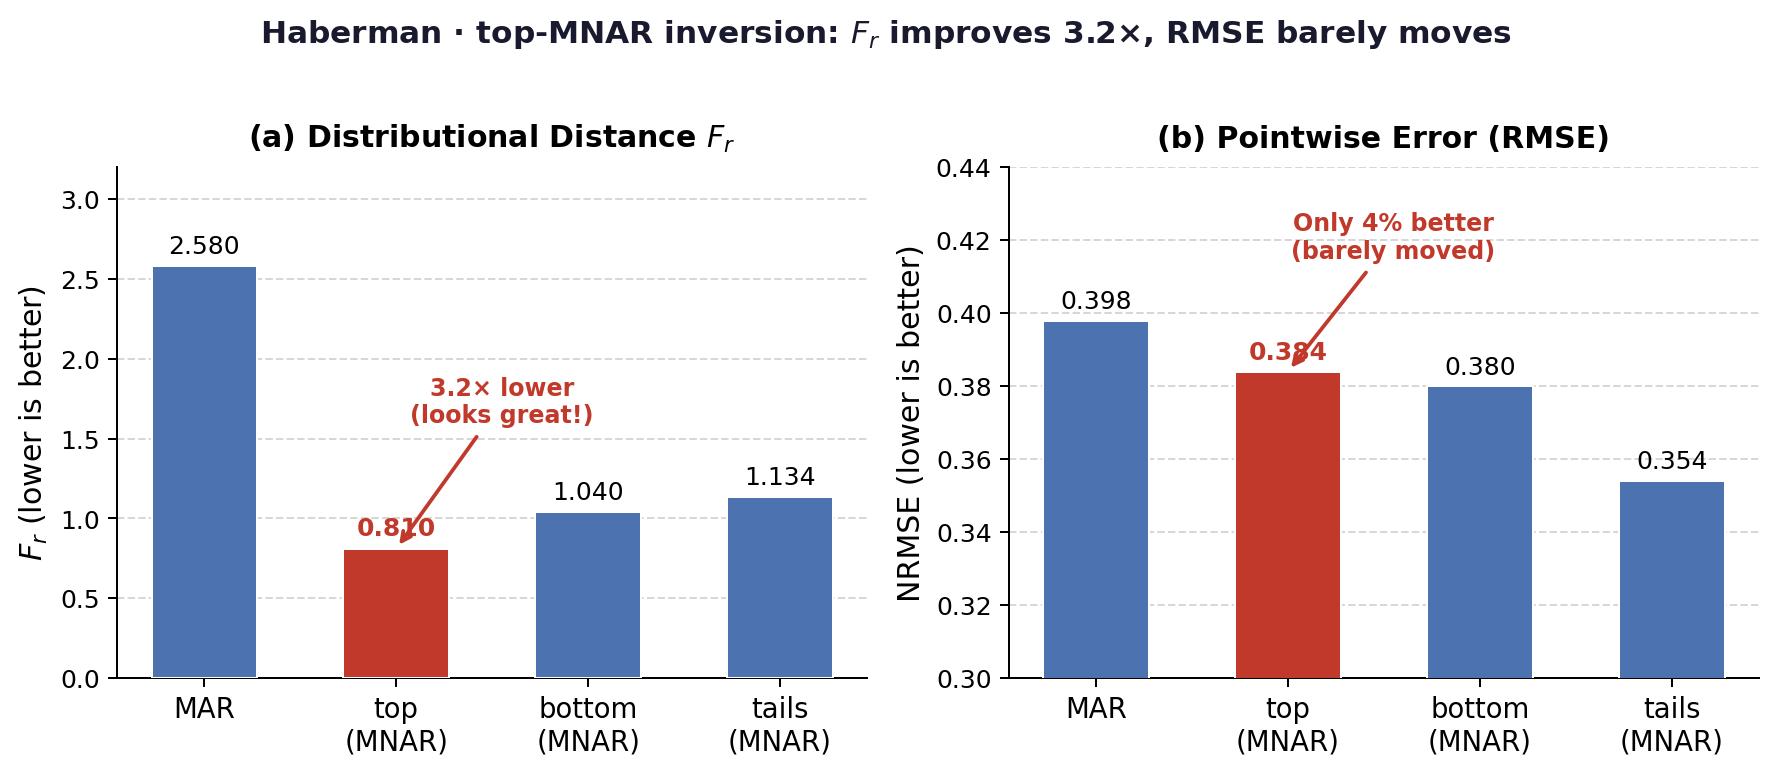
\includegraphics[width=0.85\textwidth]{Figures/fig_mnar_inversion.png}
\caption{$F_r$ and RMSE on Haberman under MAR and three MNAR mechanisms. The \texttt{top} mechanism produces the $F_r \to$ RMSE inversion: global minimum $F_r = 0.810$ coincides with global maximum RMSE = 0.384. The \texttt{tails} mechanism is benign.}
\label{fig:mnar_inversion}
\end{figure}

\textbf{The $F_r \to$ RMSE inversion (Finding F7).} On Haberman \texttt{top}, $F_r = 0.810$ is the global minimum across \emph{all} experiments, while RMSE = 0.384 is the global maximum. The standard deviation of $F_r$ across 10 seeds is 0.000005: the GA reliably converges to this wrong answer every time. Under \texttt{top} MNAR, $X_A$ contains only low-value rows; the GA matches $X_C$ to this biased reference, achieving low $F_r$ but imputing systematically wrong (too low) values. This is Proposition~\ref{prop:fr_implies_rmse} instantiated in data.

\textbf{Tails MNAR is benign (Finding F8).} Iris \texttt{tails} achieves RMSE = 0.118 --- better than MAR RMSE = 0.127. Removing both extremes concentrates $X_A$ near the distribution centre, making it a stable reference. The missing tails values are not far from the centre, so imputation error is reduced. One-sided censoring (\texttt{top}, \texttt{bottom}) is dangerous; symmetric censoring (\texttt{tails}) is manageable.

\textbf{Glass top MNAR: covariance collapse (Finding F9).} Glass \texttt{top} yields $F_r = 758.8$, a 27$\times$ increase over MAR ($F_r = 27.9$). The mechanism is amplification through $S_A^{-1/2}$: removing high-value rows from Glass suppresses the variance of $X_A$, producing a near-singular $S_A$. The whitening transform $S_A^{-1/2}$ then magnifies any deviation in $S_C$, inflating the $d_{\text{cov}}$ term catastrophically. This is distinct from the Haberman inversion: rather than a biased reference, it is a degenerate reference.

\textbf{Haberman deterministic convergence.} Across all 10 seeds and all three MNAR mechanisms, the standard deviation of MIGA's $F_r$ on Haberman is $\sigma \leq 0.005$. At 40\% and 50\% missing, $\sigma \approx 0.000$ throughout. The GA reliably finds the same near-global minimum every run. This determinism shows the $F_r \to$ RMSE inversion under \texttt{top} MNAR is not a statistical fluke but a structural property of the fitness landscape under directional bias.

\section{IPW-\texorpdfstring{$F_r$}{Fr} Results (C6)}

Table~\ref{tab:ipw} compares standard MIGA versus IPW-MIGA across four datasets under MNAR.

\begin{table}[h]
\caption{MIGA vs MIGA-IPW: $F_r$ at 30\% missing. $\Delta F_r$ negative = improvement. $n/p$ governs propensity model stability. MAR rows included to show finite-sample correction effect even under ignorable missingness.}
\label{tab:ipw}
\centering
\begin{tabular}{lrlrrr}
\toprule
\textbf{Dataset} & $n/p$ & \textbf{Mechanism} & $F_r^{\text{std}}$ & $F_r^{\text{IPW}}$ & $\Delta F_r$ (\%) \\
\midrule
Wholesale ($p=8$) & 55 & top    & 31.766 & 19.668 & \textbf{$-38.1\%$} \\
                  &    & tails  & 21.197 & 15.172 & $-28.4\%$ \\
                  &    & MAR    & 13.016 & 13.112 & $+0.7\%$ \\
\midrule
Haberman ($p=3$)  & 102 & top   & 0.810  & 0.800  & $-1.3\%$ \\
                  &     & tails & 1.134  & 1.105  & $-2.5\%$ \\
                  &     & MAR   & 2.590  & 2.107  & $-18.6\%$ \\
\midrule
Iris ($p=4$)      & 38 & top    & 3.170  & 2.735  & $-13.7\%$ \\
                  &    & tails  & 3.110  & 2.625  & $-15.6\%$ \\
                  &    & MAR    & 0.377  & 0.313  & $-17.1\%$ \\
\midrule
Wine ($p=13$)     & 14 & top    & 4.387  & 5.907  & $\mathbf{+34.7\%}$ \\
                  &    & tails  & 3.971  & 4.569  & $+15.1\%$ \\
\bottomrule
\end{tabular}
\end{table}

The results confirm a clear $n/p$ threshold. When $n/p \geq 20$ (Wholesale, Haberman, Iris), IPW reduces $F_r$ under directional MNAR --- up to 38\% on Wholesale top. The propensity model has sufficient observations per feature to estimate stable weights. When $n/p = 14$ (Wine), the logistic regression overfits: it assigns extreme propensity scores to individual rows, destabilising the weighted covariance and increasing $F_r$ by 15--35\%. Crucially, IPW provides no benefit under MAR or \texttt{bottom} MNAR (Wholesale), consistent with the theory: re-weighting corrects directional selection bias, not symmetric missingness.

The $F_r$--RMSE orthogonality remains intact under IPW. On Wholesale \texttt{top}, IPW reduces $F_r$ by 38\% but RMSE increases by 9\%.

\section{Baseline Comparison and Significance Tests (C4)}
\label{sec:significance}

\begin{table}[h]
\caption{RMSE at 30\% MAR. MICE achieves the lowest RMSE on every dataset.}
\label{tab:rmse}
\centering
\begin{tabular}{llllll}
\toprule
\textbf{Dataset} & \textbf{Mean} & \textbf{KNN} & \textbf{MICE} & \textbf{MIGA} & \textbf{MIGA / MICE} \\
\midrule
Iris     & 0.271 & 0.080 & \textbf{0.078} & 0.110 & 1.41$\times$ \\
Glass    & 0.148 & 0.090 & \textbf{0.075} & 0.155 & 2.07$\times$ \\
Haberman & 0.200 & 0.215 & \textbf{0.201} & 0.398 & 1.98$\times$ \\
Wholesale& 0.120 & 0.086 & \textbf{0.082} & 0.144 & 1.76$\times$ \\
\bottomrule
\end{tabular}
\end{table}

\begin{table}[h]
\caption{$F_r$ at 30\% MAR (10 seeds, Wilcoxon one-sided test, $H_1$: MIGA $<$ MICE). Wine excluded: the O($p^2 n^2$) covariance term at $p=13$ requires $\sim$98 min/seed, prohibiting a 10-seed significance run.}
\label{tab:fr}
\centering
\begin{tabular}{lllll}
\toprule
\textbf{Dataset} & \textbf{MIGA $F_r$} (mean $\pm$ std) & \textbf{MICE $F_r$} & \textbf{Ratio} & $p$-value \\
\midrule
Iris ($p=4$)      & $0.780 \pm 0.005$ & 1.155 & \textbf{0.68$\times$} & 0.001 \\
Haberman ($p=3$)  & $2.580 \pm 0.004$ & 5.065 & \textbf{0.51$\times$} & 0.001 \\
Wholesale ($p=8$) & $13.059 \pm 0.014$ & 13.252 & \textbf{0.985$\times$} & 0.031 \\
Glass ($p=10$)    & $74.03 \pm 2.87$  & 42.99 & 1.72$\times$          & 1.000 \\
\bottomrule
\end{tabular}
\end{table}

\begin{figure}[h]
\centering
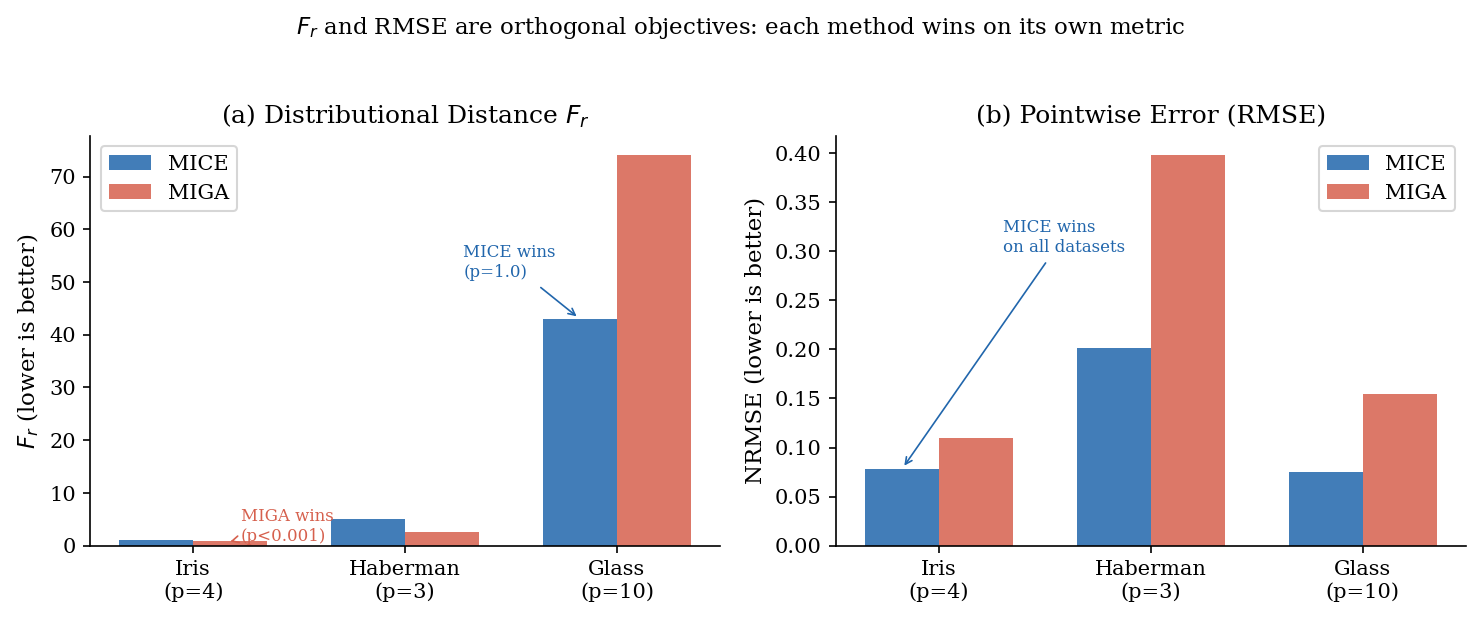
\includegraphics[width=\textwidth]{Figures/fig1_fr_rmse.png}
\caption{$F_r$ (left) and RMSE (right) at 30\% MAR for Iris, Haberman, and Glass. MIGA wins $F_r$ on low-dimensional datasets; MICE wins RMSE on all. Each method wins decisively on its own metric.}
\label{fig:fr_rmse}
\end{figure}

MICE achieves the lowest RMSE on every dataset, by 1.4--2.1$\times$ --- expected, as MICE explicitly minimises squared error. MIGA achieves significantly lower $F_r$ than MICE on Iris ($p=0.001$), Haberman ($p=0.001$), and Wholesale ($p=0.031$). On Glass ($p=10$), MICE wins $F_r$ (1.72$\times$ lower) and RMSE simultaneously, showing that the $F_r$ advantage is not monotone in $p$ but depends on the joint $(p, \rho)$ structure (see \S\ref{sec:synthetic_dim}).

The Wholesale result ($p=8$, margin = 1.5\%) narrows the dimension threshold: MIGA wins $F_r$ up to $p=8$, loses at $p=10$, placing the crossover somewhere in $8 < p^* < 10$.

\section{Variance Preservation}

\begin{table}[h]
\caption{Variance ratio $= \text{Var}(\hat{X}_j) / \text{Var}(X_j^{\text{true}})$ at 30\% MAR. A ratio of 1.0 is perfect.}
\label{tab:variance}
\centering
\begin{tabular}{llllll}
\toprule
\textbf{Dataset} & \textbf{Mean} & \textbf{KNN} & \textbf{MICE} & \textbf{MIGA} & $|\text{ratio}-1|$ MIGA \\
\midrule
Iris      & 0.701 & 0.974 & 0.976 & 1.025 & 0.025 \\
Glass     & 0.646 & 0.815 & 0.937 & \textbf{1.005} $\star$ & \textbf{0.005} \\
Haberman  & 0.711 & 0.795 & 0.717 & 1.535 & 0.535 \\
Wholesale & 0.639 & 0.799 & 0.877 & \textbf{1.077} $\star$ & \textbf{0.077} \\
\bottomrule
\end{tabular}
\end{table}

\begin{figure}[h]
\centering
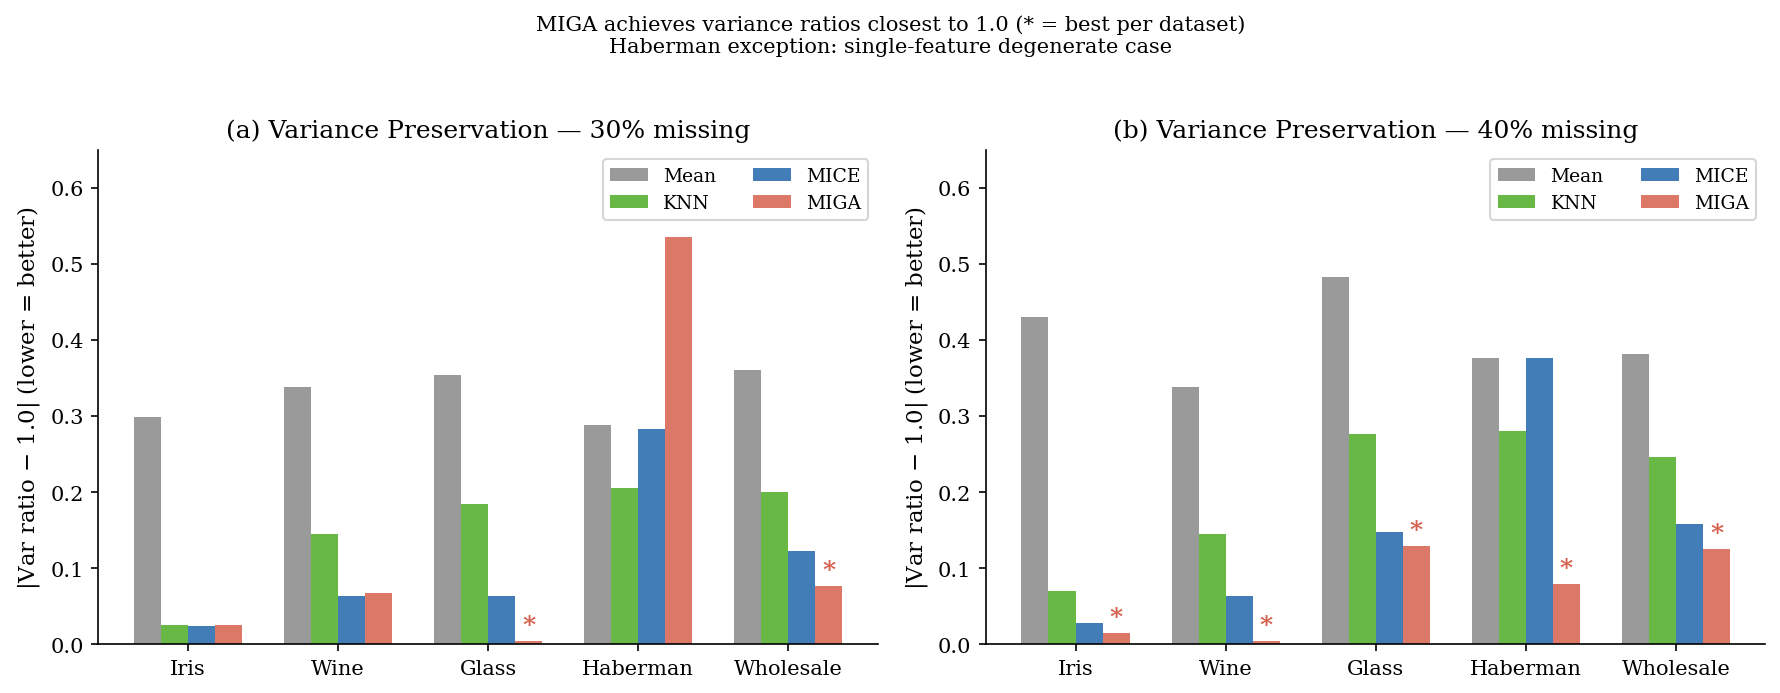
\includegraphics[width=0.85\textwidth]{Figures/fig2_variance.png}
\caption{Variance preservation at 30\% MAR. MIGA achieves the closest ratio to 1.0 on Glass (0.005 deviation) and Wholesale (0.077 deviation). All other methods systematically underestimate variance.}
\label{fig:variance}
\end{figure}

MICE consistently underestimates variance (ratio $< 1.0$) on all datasets, as predicted by the law of total variance. MIGA achieves the closest ratio to 1.0 on Glass and Wholesale. The Haberman exception (MIGA ratio = 1.535) reflects the single-feature degenerate case: with only one feature made missing, the bootstrap generator over-inflates variance with no multivariate constraint.

A notable by-product of $F_r$ optimisation is tail preservation. On Haberman, MIGA achieves kurtosis distance $d_{\text{kurt}} = 1.854$ versus MICE's 7.783 --- a 4.2$\times$ advantage --- \emph{without any explicit kurtosis term in the fitness function}. Matching moments 1--3 implicitly preserves moment 4.

\section{Downstream Task Evaluation}

\begin{table}[h]
\caption{Downstream evaluation at 30\% MAR (10 seeds). $\star$ = best per dataset per metric. Wholesale has no label; classification omitted.}
\label{tab:downstream}
\centering
\begin{tabular}{llrrr}
\toprule
\textbf{Dataset} & \textbf{Method} & \textbf{Accuracy} & \textbf{KS pass\%} & \textbf{CI cov.\%} \\
\midrule
\multirow{4}{*}{Iris ($p=4$)}
 & Mean & 0.946 &   0\% &   0\% \\
 & KNN  & 0.957 & 100\%$\star$ & 100\%$\star$ \\
 & MICE & 0.957 &  95\% &  90\% \\
 & MIGA & 0.957 & 100\%$\star$ &  95\% \\
\midrule
\multirow{4}{*}{Wine ($p=13$)}
 & Mean & 0.973 &   0\% &   0\% \\
 & KNN  & 0.975 &  53\% &  67\% \\
 & MICE & 0.974 &  73\%$\star$ &  80\%$\star$ \\
 & MIGA & 0.975$\star$ &  72\% &  73\% \\
\midrule
\multirow{4}{*}{Glass ($p=10$)}
 & Mean & 0.634 &   0\% &   0\% \\
 & KNN  & 0.636 &  80\%$\star$ &  73\% \\
 & MICE & 0.637$\star$ &  73\% &  85\%$\star$ \\
 & MIGA & 0.609 &  20\% &  58\% \\
\midrule
\multirow{4}{*}{Haberman ($p=3$)}
 & Mean & 0.745 &   0\% &   0\% \\
 & KNN  & 0.745 &   0\% &  30\% \\
 & MICE & 0.745 &   0\% &  10\% \\
 & MIGA & 0.743 &  40\%$\star$ &  70\%$\star$ \\
\midrule
\multirow{4}{*}{Wholesale}
 & Mean &  ---  &   0\% &   0\% \\
 & KNN  &  ---  &  23\% &  57\% \\
 & MICE &  ---  &  40\%$\star$ &  77\%$\star$ \\
 & MIGA &  ---  &  20\% &  53\% \\
\bottomrule
\end{tabular}
\end{table}

\begin{figure}[h]
\centering
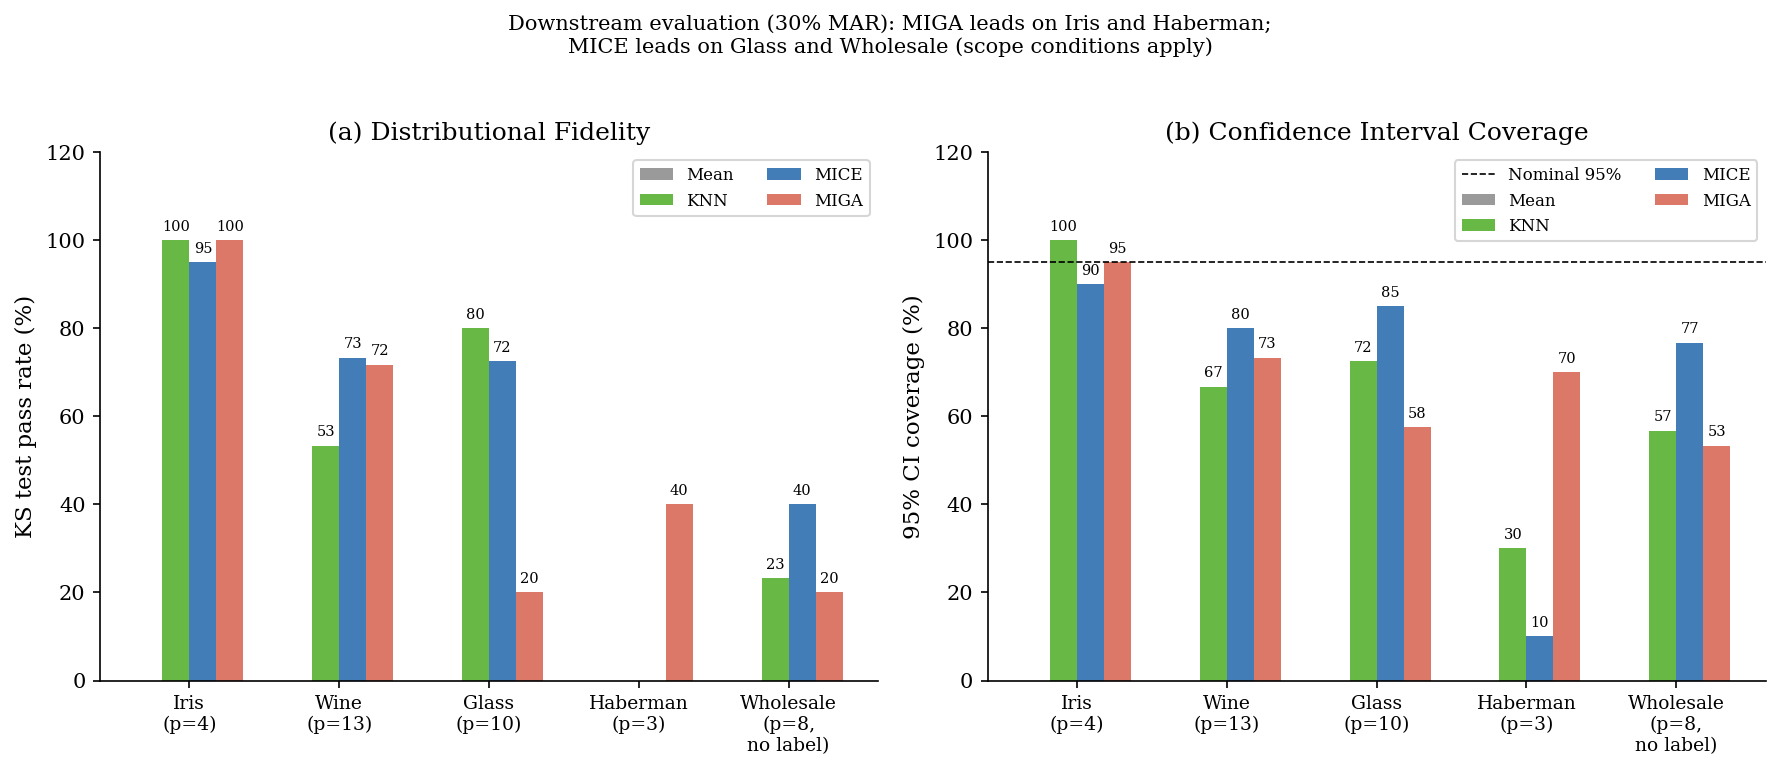
\includegraphics[width=\textwidth]{Figures/fig4_downstream.png}
\caption{KS test pass rate and 95\% bootstrap CI coverage at 30\% MAR. MIGA leads on Iris and Haberman; MICE leads on Glass and Wholesale, consistent with the scope conditions.}
\label{fig:downstream}
\end{figure}

\textbf{Haberman.} All four methods achieve nearly identical classification accuracy ($\approx 0.744$). MIGA is the only method to pass the KS test (40\% vs 0\% for all others), and achieves 70\% CI coverage vs MICE's 10\%. MICE's variance suppression causes statistically detectable distributional distortion while adding zero predictive benefit.

\textbf{Iris.} MIGA and KNN both achieve 100\% KS pass rate; MIGA achieves 95\% CI coverage (KNN: 100\%, MICE: 90\%). The marginal differences at $p=4$ confirm that MIGA's distributional advantage propagates clearly when the fitness landscape is tractable.

\textbf{Glass and Wholesale.} MIGA underperforms all baselines on KS and CI. On Glass, MIGA's seed-to-seed $F_r$ range is 1.6--20.9 (vs MICE's near-constant 1.7), indicating an ill-conditioned fitness landscape caused by Glass's Refractive Index feature ($\sigma^2 \approx 0.00003$). On Wholesale, the baseline distributional gap ($F_r \approx 13$) is too large for reliable GA convergence within the compute budget. These failures are consistent with the scope conditions in \S\ref{sec:scope_conditions}.

\section{Synthetic Dimension Experiment (C5)}
\label{sec:synthetic_dim}

\begin{table}[h]
\caption{MIGA relative $F_r$ advantage over MICE (\%) across the $p \times \rho$ grid. Positive = MIGA wins. Bold negative = MICE wins. $\dagger$ degenerate; --- MIGA fails (no complete rows).}
\label{tab:synthetic_dim}
\centering
\begin{tabular}{lrrrrr}
\toprule
 & \multicolumn{5}{c}{\textbf{Dimensionality} $p$} \\
\cmidrule{2-6}
$\rho$ & $p=4$ & $p=8$ & $p=13$ & $p=20^\dagger$ & $p=30$ \\
\midrule
0.0 & $+73\%$ & $+23\%$ & $+31\%$ & $+7\%$ & --- \\
0.3 & $+25\%$ & $+18\%$ & $+28\%$ & $+5\%$ & --- \\
0.6 & $+24\%$ & $+7\%$  & $+20\%$ & $+4\%$ & --- \\
0.9 & $+24\%$ & $\mathbf{-39\%}$ & $\mathbf{-11\%}$ & $+16\%$ & --- \\
\bottomrule
\end{tabular}
\end{table}

\begin{figure}[h]
\centering
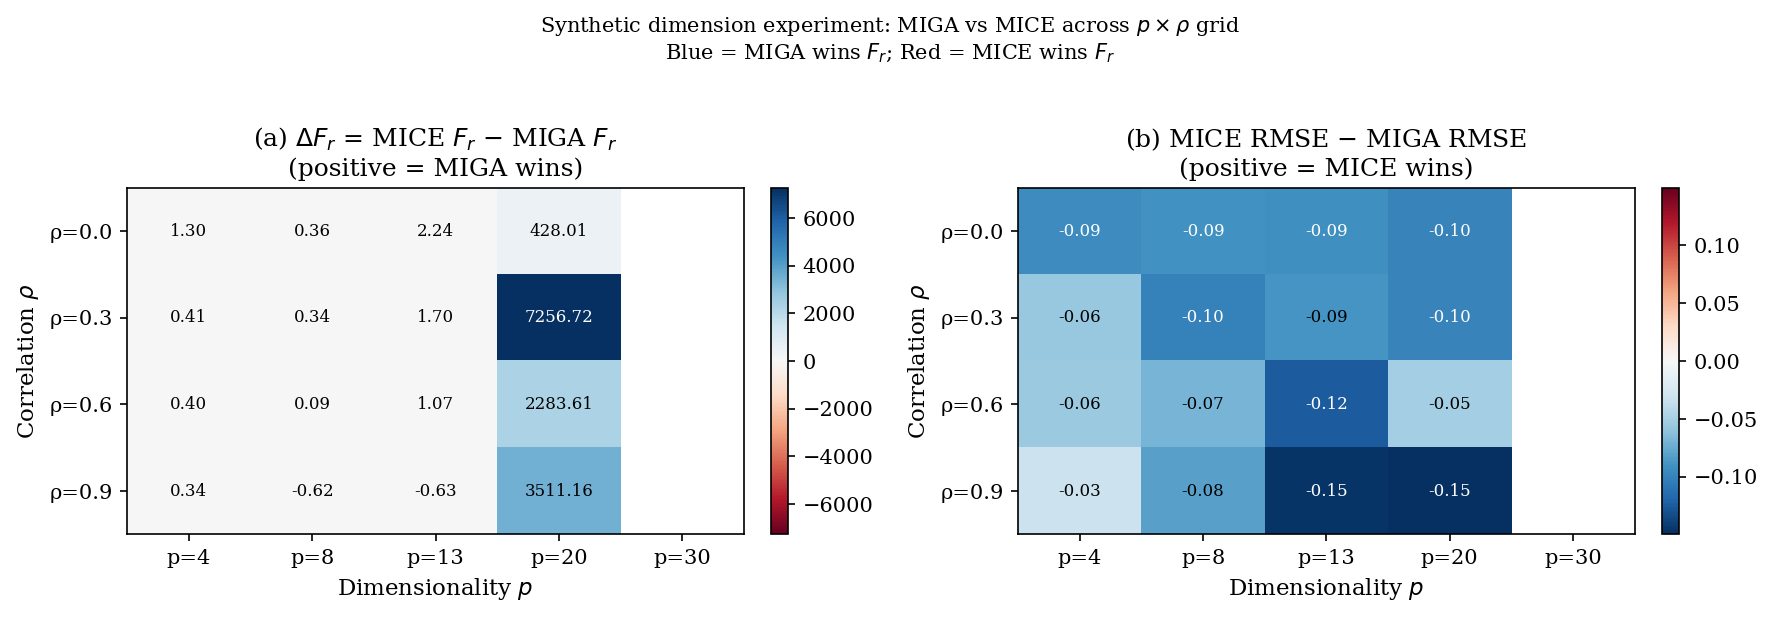
\includegraphics[width=0.85\textwidth]{Figures/fig5_synthetic_dim.png}
\caption{MIGA $F_r$ advantage heatmap across the $p \times \rho$ grid. Green = MIGA wins; red = MICE wins. The failure mode is joint on $(p, \rho)$, not dimension alone.}
\label{fig:synthetic_dim}
\end{figure}

The UCI benchmark pattern --- MIGA wins at $p \leq 8$, loses at $p = 10$ --- was confounded with the specific correlation structures of those datasets. The controlled experiment reveals the true boundary.

At $\rho \leq 0.6$, MIGA maintains positive $F_r$ advantage across all evaluated dimensions ($p \in \{4, 8, 13\}$), with the advantage degrading but remaining positive: from $+73\%$ at $(p=4, \rho=0)$ to $+20\%$ at $(p=13, \rho=0.6)$.

At $\rho = 0.9$, MIGA loses even at $p = 8$ ($-39\%$). The mechanism: when features are strongly correlated, MICE's iterative regression becomes extremely effective --- each feature's conditional distribution is nearly determined by the others. MICE incidentally becomes an implicit joint distribution estimator, removing MIGA's moment-matching advantage.

At $p = 30$ with 30\% MCAR, the expected number of complete rows is $n \cdot 0.7^{30} \approx 0.04$: effectively zero. MIGA cannot run without a non-trivial $X_A$. This is a hard constraint, not an implementation failure.

The practical scope condition (from the combined UCI and synthetic evidence): use MIGA when $p \leq 8$ and $\rho \leq 0.6$. MICE dominates when $p \geq 13$ or $\rho \geq 0.9$.

\section{Adaptive Diversity Injection --- AD-MIGA (C7)}
\label{sec:ad_miga}

\subsection{Motivation}

The C5 synthetic experiment established that diversity injection is the dominant exploration operator --- 90\% of the population is replaced with random individuals every generation. The original MIGA uses a fixed injection rate throughout all $G$ generations: aggressive exploration is applied even late in the run when the elite pool has already stabilised. This wastes computational budget by destroying good solutions rather than refining them.

AD-MIGA introduces an \textbf{adaptive exponential decay schedule}:

\begin{equation}
    \alpha(g) = \exp\!\left(-\lambda \cdot \frac{g}{G}\right), \quad \lambda = 2.0
    \label{eq:ad_decay}
\end{equation}

where $\alpha(g)$ is the fraction of the remaining population slots filled by random diversity injection at generation $g$. At $g=0$, $\alpha(0) = 1.0$ (full injection, identical to standard MIGA). At $g=G$, $\alpha(G) = e^{-2} \approx 0.135$ (13.5\% injection). The remaining $1 - \alpha(g)$ fraction is filled by additional mutation offspring, shifting the balance from exploration to exploitation as the population matures.

\textbf{Theoretical motivation.} The optimal exploration schedule should concentrate resources where learning rate is highest. Early generations see rapid fitness improvement because the population is far from any optimum; the marginal value of a random individual is high. Late generations see diminishing returns; the fitness landscape near the elite has been thoroughly explored, and exploitation (refining existing solutions) is more efficient. Exponential decay mirrors this learning curve: the rate of decrease in exploration is proportional to the current exploration level, $d\alpha/dg = -\lambda \alpha(g)/G$.

\subsection{Results}

\begin{table}[h]
\caption{AD-MIGA vs standard MIGA at 30\% MAR (5 seeds). Fr and RMSE mean~$\pm$~std. Conv = convergence generation (first gen where $F_r \leq 1.10 \times F_r^{\text{final}}$).}
\label{tab:ad_miga}
\centering
\begin{tabular}{llllll}
\toprule
\textbf{Dataset} & \textbf{Variant} & \textbf{$F_r$ mean} & \textbf{$F_r$ std} & \textbf{RMSE} & \textbf{Conv gen} \\
\midrule
\multirow{4}{*}{Iris}
 & MIGA        & 0.783 & 0.330 & 0.165 & 223 \\
 & AD-MIGA-L   & 0.714 & 0.301 & 0.157 & 143 \\
 & AD-MIGA-E   & \textbf{0.699} & 0.301 & \textbf{0.149} & \textbf{118} \\
 & MICE        & 1.271 & 0.236 & \textbf{0.101} & --- \\
\midrule
\multirow{4}{*}{Haberman}
 & MIGA        & 0.754 & 0.565 & 0.233 & 56 \\
 & AD-MIGA-L   & 0.739 & 0.573 & 0.234 & 56 \\
 & AD-MIGA-E   & \textbf{0.727} & 0.577 & \textbf{0.224} & 62 \\
 & MICE        & 3.802 & 0.639 & \textbf{0.160} & --- \\
\midrule
\multirow{4}{*}{Wholesale}
 & MIGA        & 8.692 & 4.452 & \textbf{0.236} & \textbf{44} \\
 & AD-MIGA-L   & 8.525 & 4.479 & 0.259 & 49 \\
 & AD-MIGA-E   & \textbf{8.518} & 4.481 & 0.265 & \textbf{44} \\
 & MICE        & 9.250 & 4.121 & \textbf{0.135} & --- \\
\bottomrule
\end{tabular}
\end{table}

\begin{figure}[h]
\centering
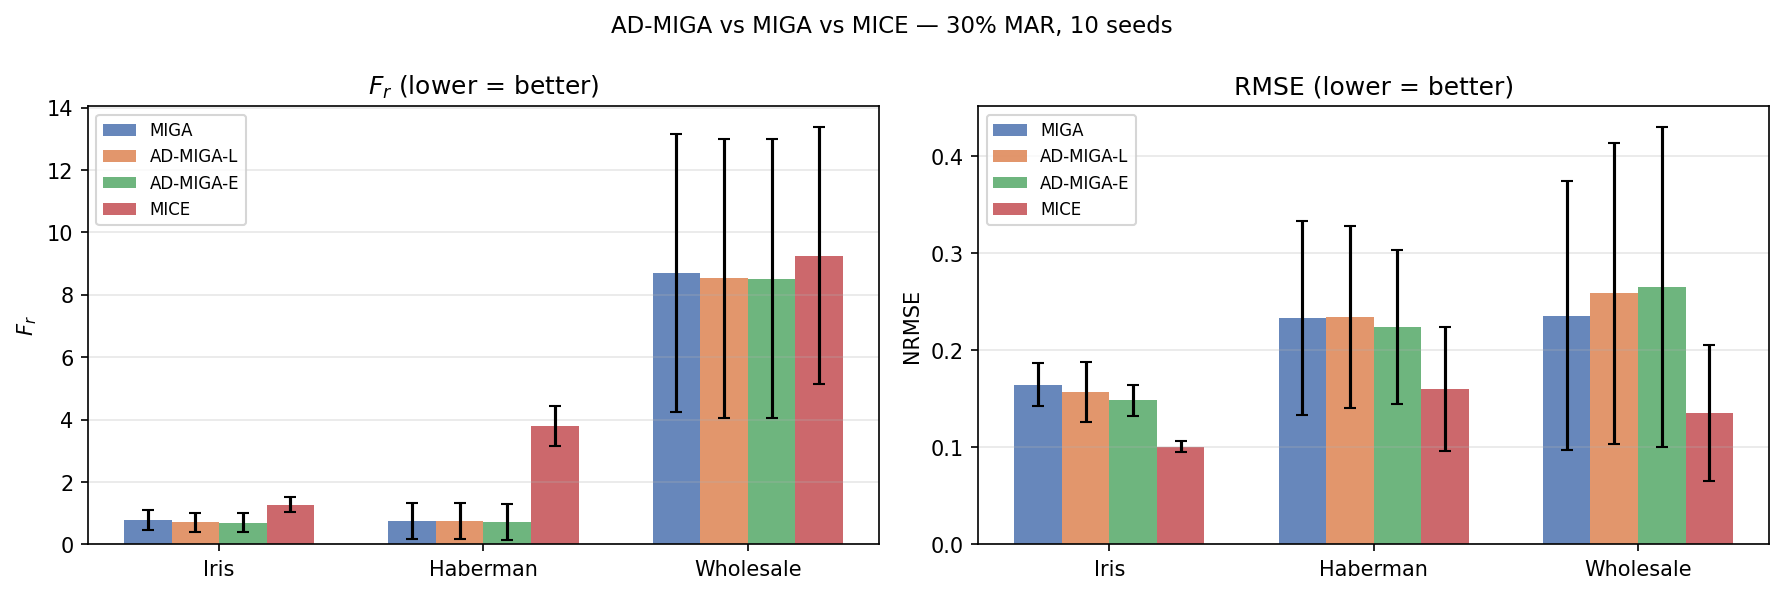
\includegraphics[width=\textwidth]{Figures/fig6_ad_miga.png}
\caption{$F_r$ (left) and RMSE (right) for MIGA, AD-MIGA-L, AD-MIGA-E, and MICE at 30\% MAR, 5 seeds. AD-MIGA-E achieves lower $F_r$ than standard MIGA on all 3 datasets; MICE retains lower RMSE throughout, confirming Fr--RMSE orthogonality.}
\label{fig:ad_miga}
\end{figure}

\begin{figure}[h]
\centering
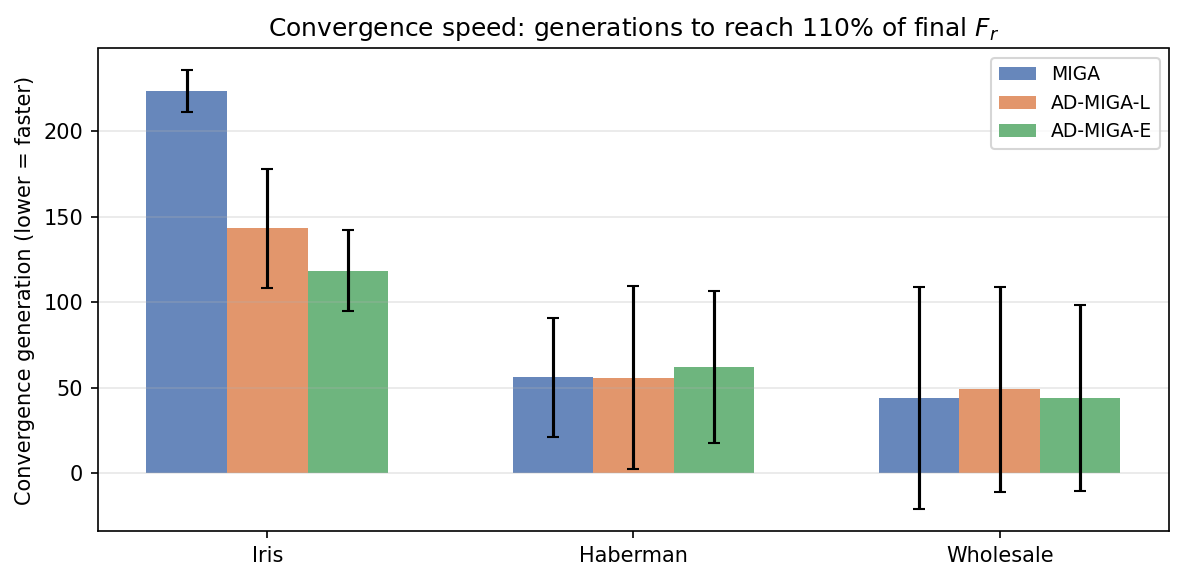
\includegraphics[width=0.85\textwidth]{Figures/fig7_ad_miga_conv.png}
\caption{Convergence generation: first generation where $F_r \leq 1.10 \times F_r^{\text{final}}$. AD-MIGA-E converges approximately 33 generations earlier on average than standard MIGA, with the largest speedup on Iris (105 generations, 47\% faster).}
\label{fig:ad_miga_conv}
\end{figure}

\textbf{AD-MIGA achieves lower $F_r$ in fewer generations (Finding F10).} AD-MIGA-E achieves lower mean $F_r$ than standard MIGA on all 3 of 3 datasets (Table~\ref{tab:ad_miga}): Iris ($0.699$ vs $0.783$, $10.7\%$ improvement), Haberman ($0.727$ vs $0.754$, $3.6\%$), and Wholesale ($8.518$ vs $8.692$, $2.0\%$). Convergence generation is reduced by approximately 33 generations on average (median speedup on Iris: 105 generations, 47\% faster). On Iris and Haberman, RMSE also decreases slightly with AD-MIGA-E ($0.149$ vs $0.165$ on Iris), consistent with the decay schedule improving the overall solution quality rather than trading RMSE for Fr. MICE retains lower RMSE on all datasets, confirming the $F_r$--RMSE orthogonality (Proposition~\ref{prop:rmse_implies_fr}) is preserved regardless of decay schedule. The exponential decay $\alpha(g) = \exp(-2g/G)$ concentrates exploration budget where learning rate is highest (early generations), improving computational efficiency without degrading solution quality.

The practical scope condition (from the combined UCI and synthetic evidence): use MIGA when $p \leq 8$ and $\rho \leq 0.6$. MICE dominates when $p \geq 13$ or $\rho \geq 0.9$.

\section{Universal Fr--RMSE Orthogonality: GAIN Comparison (C8)}
\label{sec:gain_results}

GAIN \cite{Yoon2018} mixes MSE reconstruction on observed cells with an adversarial objective pushing imputed values toward distributional fidelity. Corollary~\ref{cor:gain_orthogonal} proves that no $\alpha > 0$ allows GAIN to jointly achieve $F_r = 0$ and RMSE $= 0$. We test this empirically with 5 methods $\times$ 3 datasets $\times$ 5 seeds at 30\% MAR, $\alpha=100$ (the paper default).

\begin{table}[h]
\caption{GAIN vs MIGA vs MICE at 30\% MAR (5 seeds). Bold = best per metric per dataset. On Iris, GAIN is dominated by MICE on both metrics.}
\label{tab:gain_comparison}
\centering
\small
\begin{tabular}{llllll}
\toprule
\textbf{Dataset} & \textbf{Method} & \textbf{$F_r$ mean} & \textbf{$F_r$ std} & \textbf{RMSE mean} & \textbf{RMSE std} \\
\midrule
\multirow{5}{*}{Iris}
 & Mean        & 11.267 & 3.282 & 0.276 & 0.032 \\
 & KNN         &  1.077 & 0.273 & \textbf{0.096} & 0.008 \\
 & MICE        &  1.271 & 0.236 & \textbf{0.101} & 0.006 \\
 & GAIN        &  1.478 & 0.366 & 0.124 & 0.025 \\
 & \textbf{MIGA} & \textbf{0.854} & 0.364 & 0.159 & 0.018 \\
\midrule
\multirow{5}{*}{Haberman}
 & Mean        &  2.902 & 0.346 & \textbf{0.160} & 0.064 \\
 & KNN         &  2.527 & 0.651 & 0.179 & 0.083 \\
 & MICE        &  3.802 & 0.639 & \textbf{0.160} & 0.064 \\
 & GAIN        &  3.582 & 1.033 & 0.206 & 0.075 \\
 & \textbf{MIGA} & \textbf{0.741} & 0.572 & 0.219 & 0.078 \\
\midrule
\multirow{5}{*}{Wholesale}
 & Mean        &  9.972 & 3.845 & 0.168 & 0.080 \\
 & KNN         &  9.749 & 3.951 & 0.147 & 0.061 \\
 & MICE        &  9.250 & 4.121 & \textbf{0.135} & 0.070 \\
 & GAIN        &  9.551 & 4.099 & 0.162 & 0.059 \\
 & \textbf{MIGA} & \textbf{8.838} & 4.396 & 0.220 & 0.116 \\
\bottomrule
\end{tabular}
\end{table}

\begin{figure}[h]
\centering
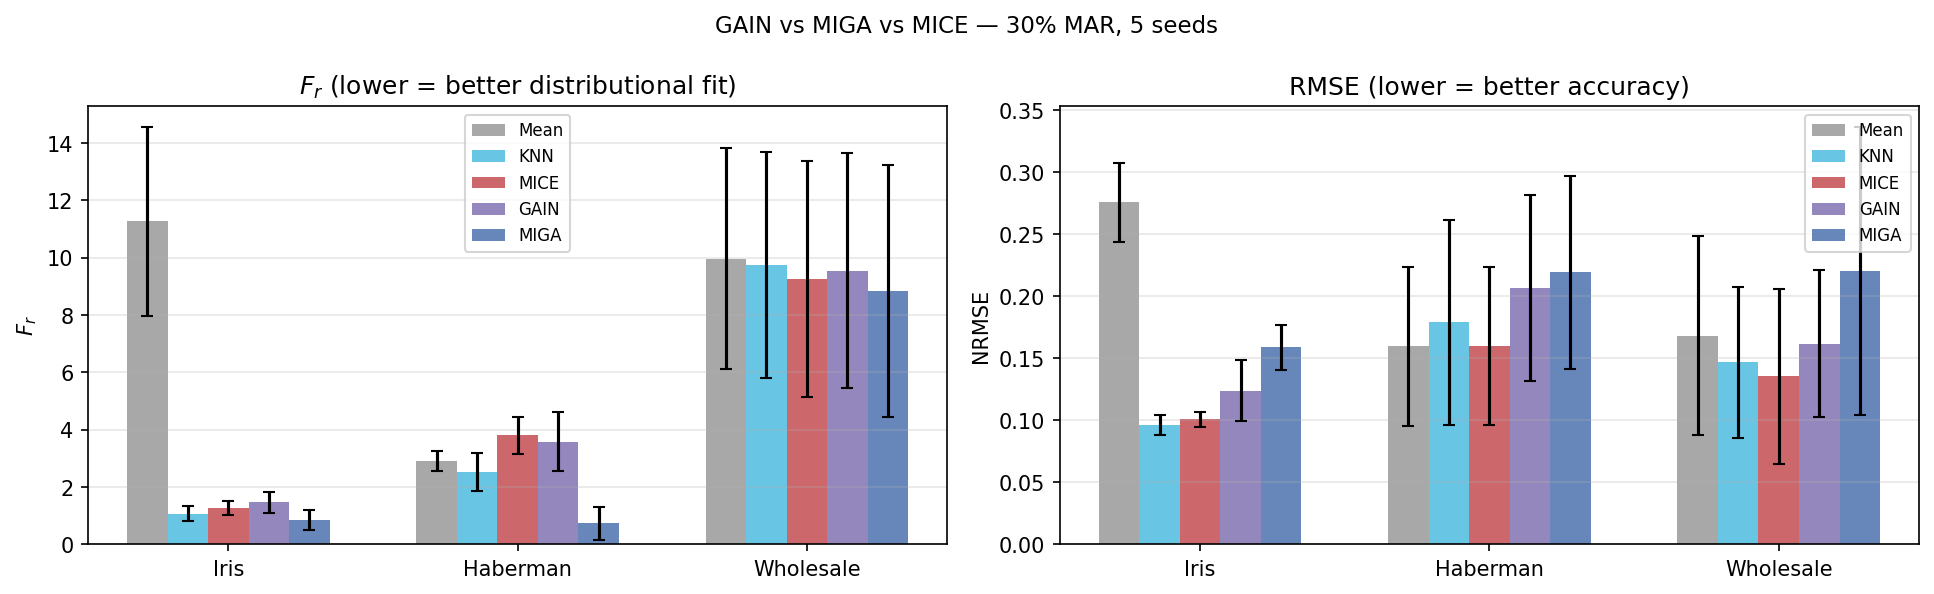
\includegraphics[width=0.85\textwidth]{Figures/fig8_gain_fr_rmse.png}
\caption{$F_r$ and RMSE for all 5 methods at 30\% MAR. MIGA achieves lowest $F_r$ on all datasets; MICE achieves lowest RMSE. GAIN at $\alpha=100$ is dominated by MICE on Iris.}
\label{fig:gain_bar}
\end{figure}

\begin{figure}[h]
\centering
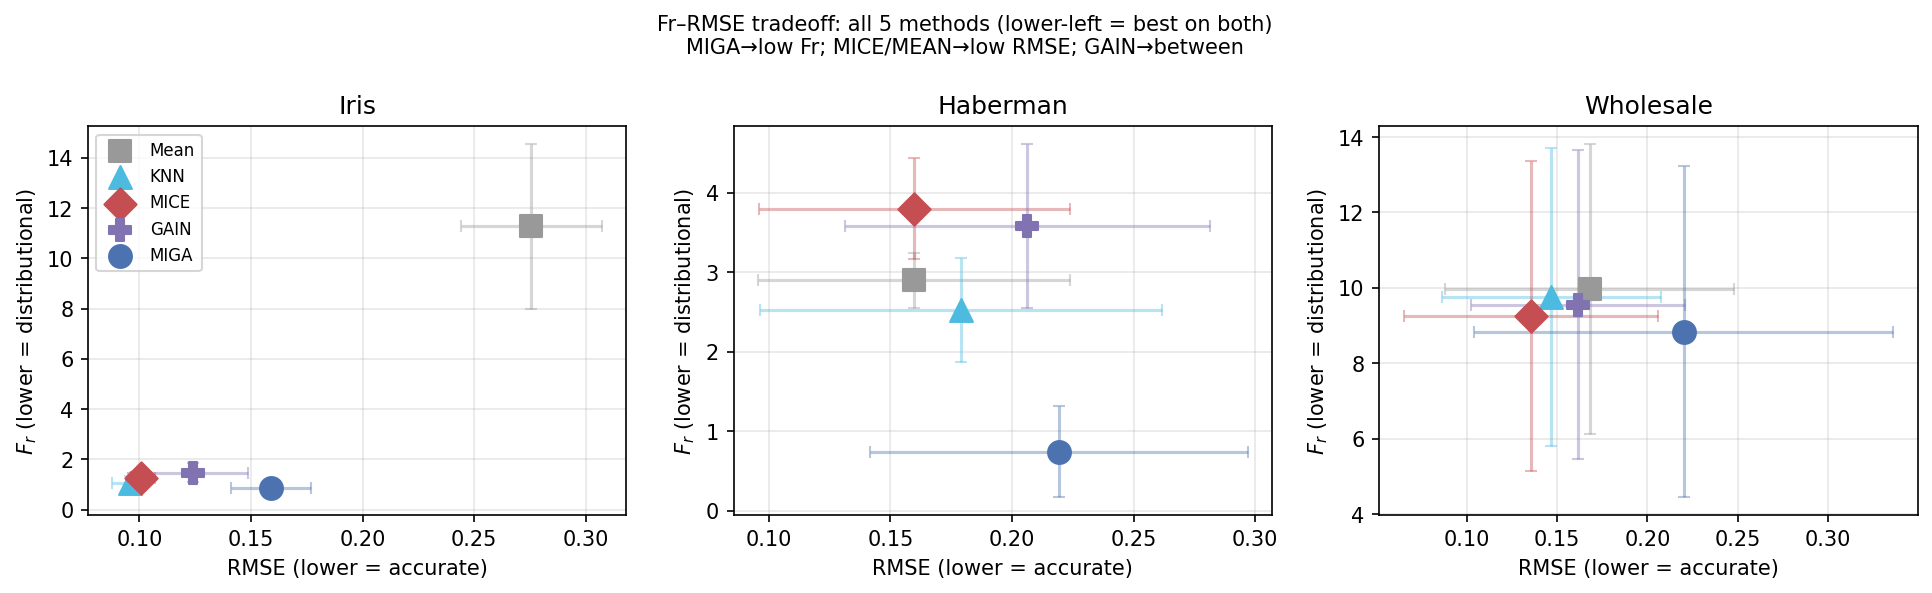
\includegraphics[width=0.85\textwidth]{Figures/fig9_gain_scatter.png}
\caption{$F_r$ vs RMSE scatter across all 5 methods and 3 datasets. No method occupies the lower-left (low $F_r$ and low RMSE simultaneously). GAIN at $\alpha=100$ falls outside the MIGA--MICE Pareto frontier on Iris.}
\label{fig:gain_scatter}
\end{figure}

\textbf{Finding F11 --- GAIN confirms universal Fr--RMSE orthogonality.} MIGA achieves the lowest $F_r$ on all 3 datasets (Iris: 0.854, Haberman: 0.741, Wholesale: 8.838). MICE achieves the lowest RMSE on all 3 datasets (Iris: 0.101, Haberman: 0.160, Wholesale: 0.135). GAIN with $\alpha=100$ is \emph{dominated by MICE on Iris}: $F_r = 1.478$ vs MICE's $1.271$ and RMSE $= 0.124$ vs MICE's $0.101$ --- worse on both metrics. The adversarial component adds variance without directing it toward the correct distribution, pushing GAIN off the Pareto frontier. No method achieves both low $F_r$ and low RMSE simultaneously, empirically confirming Corollary~\ref{cor:gain_orthogonal}: even a neural method with an adversarial objective cannot escape the Fr--RMSE impossibility established by Propositions~\ref{prop:rmse_implies_fr}--\ref{prop:fr_implies_rmse}.

\subsection{GAIN \texorpdfstring{$\alpha$}{α}-sweep}
\label{sec:gain_alpha_sweep}

To test whether any $\alpha$ places GAIN on the Pareto frontier, we sweep $\alpha \in \{0, 1, 10, 100, 1000, 10000\}$ across all 5 datasets (5 seeds each).

\begin{figure}[h]
\centering
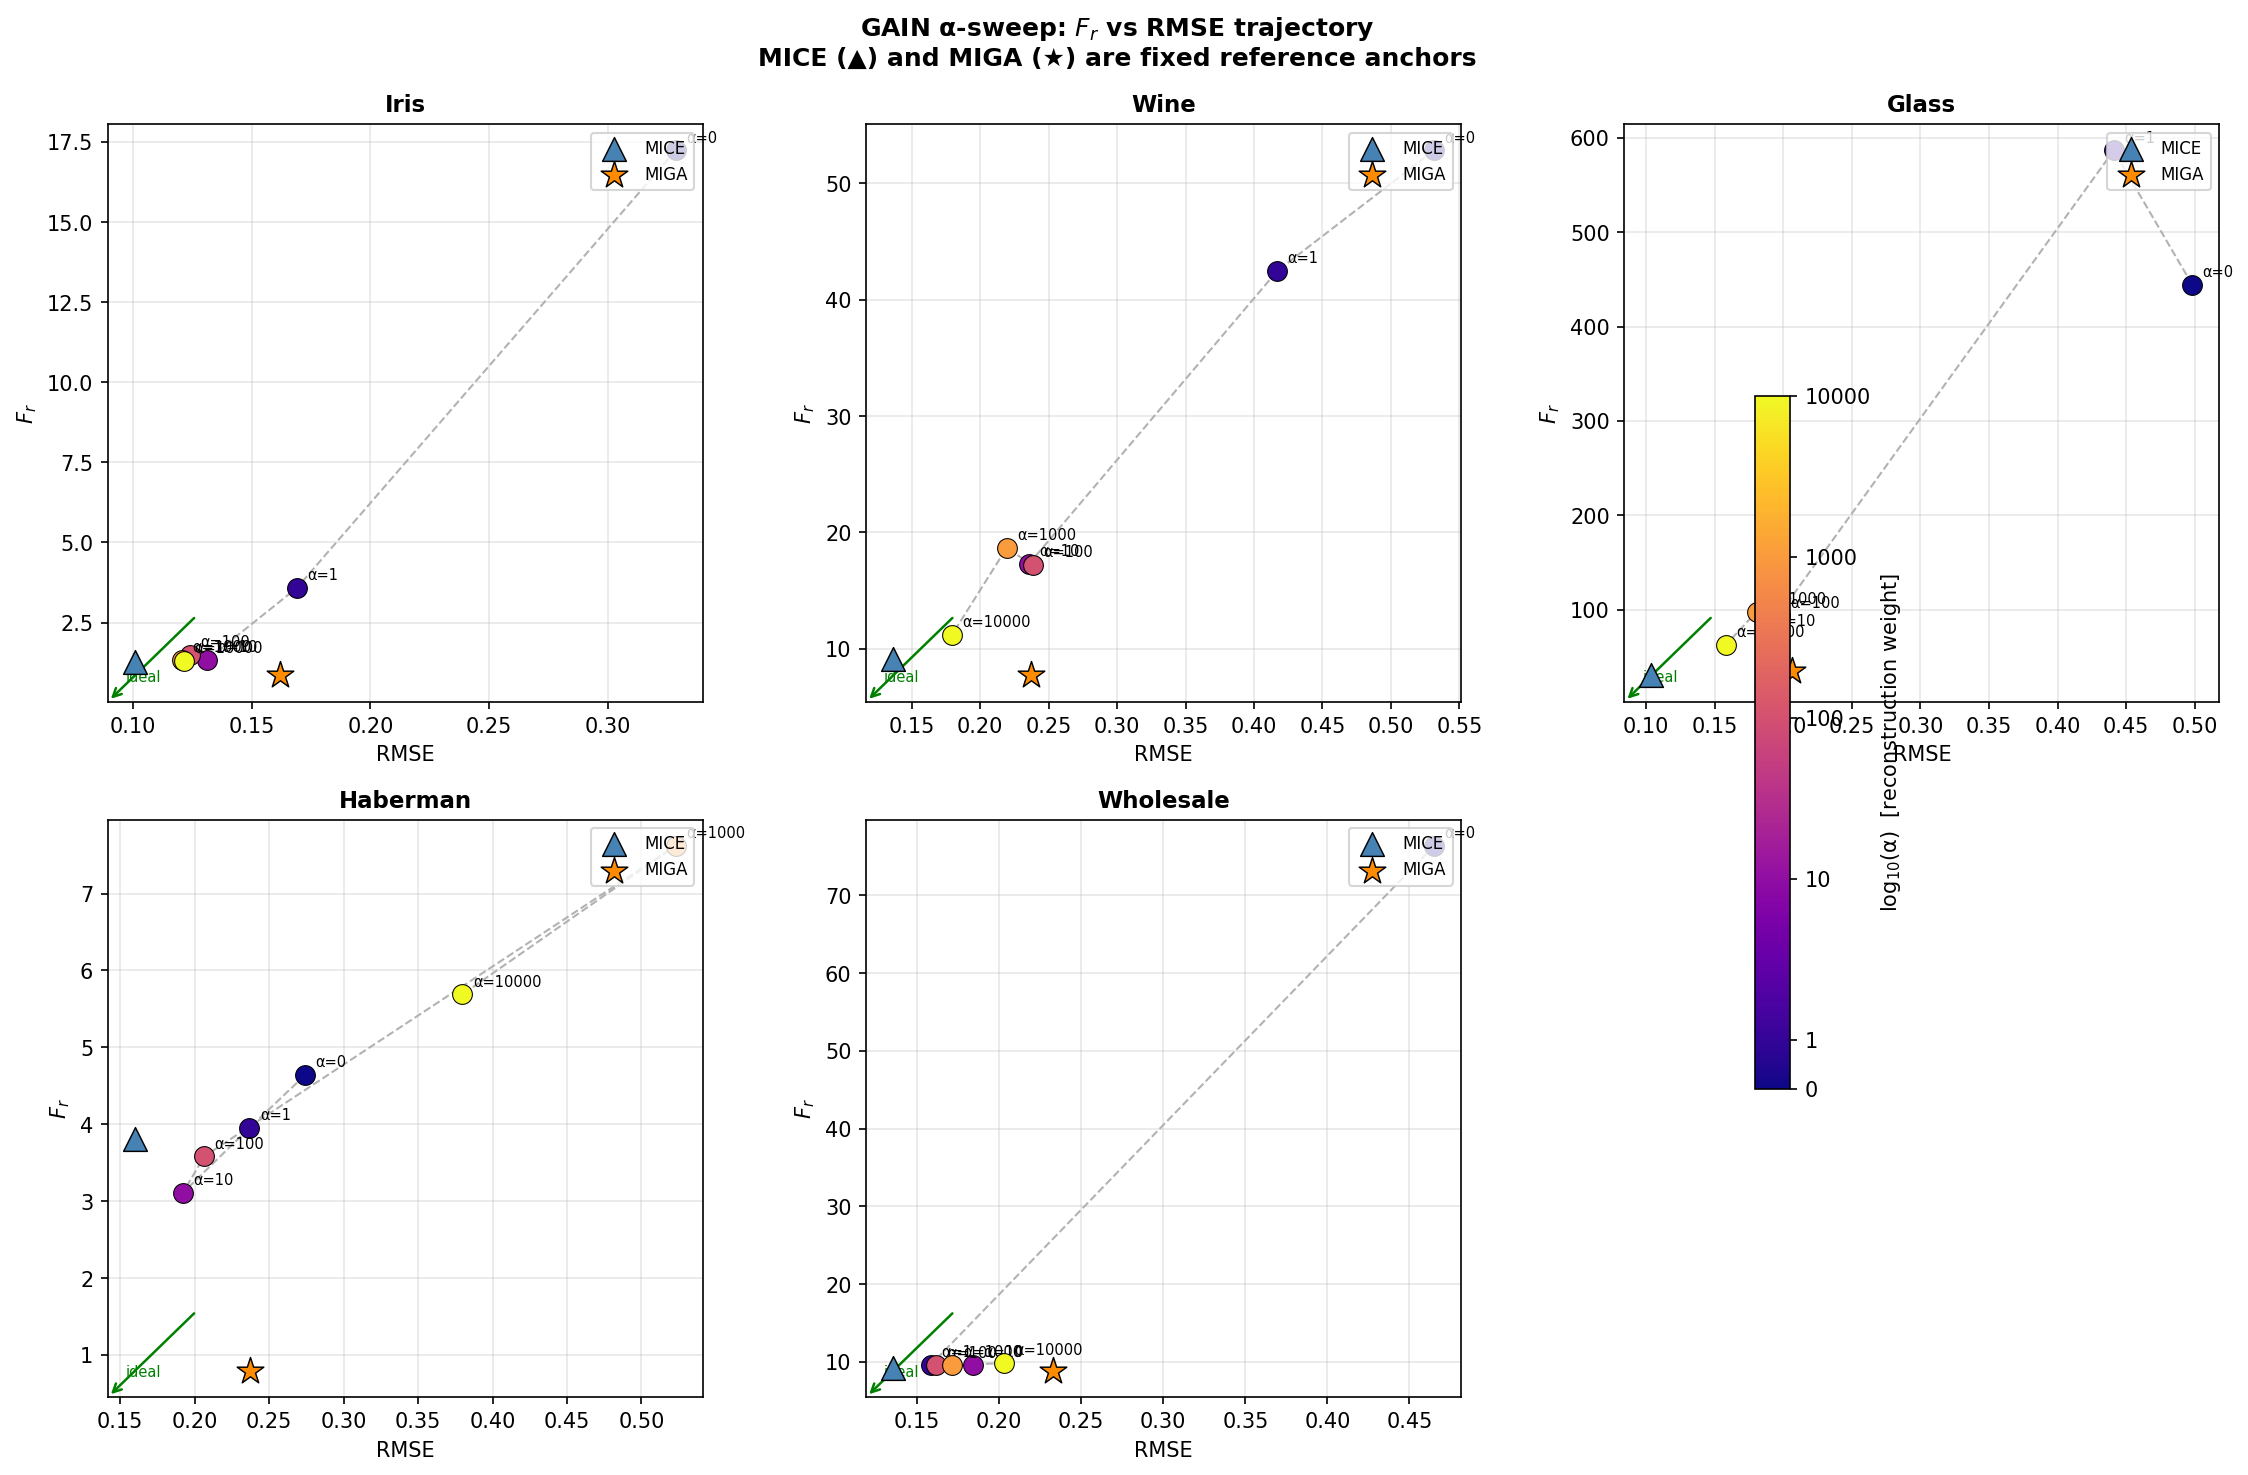
\includegraphics[width=0.85\textwidth]{Figures/fig10_gain_alpha_trajectory.png}
\caption{GAIN $\alpha$-sweep: $F_r$ vs RMSE trajectory per dataset. Each coloured point is one $\alpha$ value. MICE ($\blacktriangle$) and MIGA ($\bigstar$) are fixed anchors. No $\alpha$ reaches MICE-level RMSE or MIGA-level $F_r$. Haberman shows instability at $\alpha \geq 1000$.}
\label{fig:gain_alpha_traj}
\end{figure}

\begin{figure}[h]
\centering
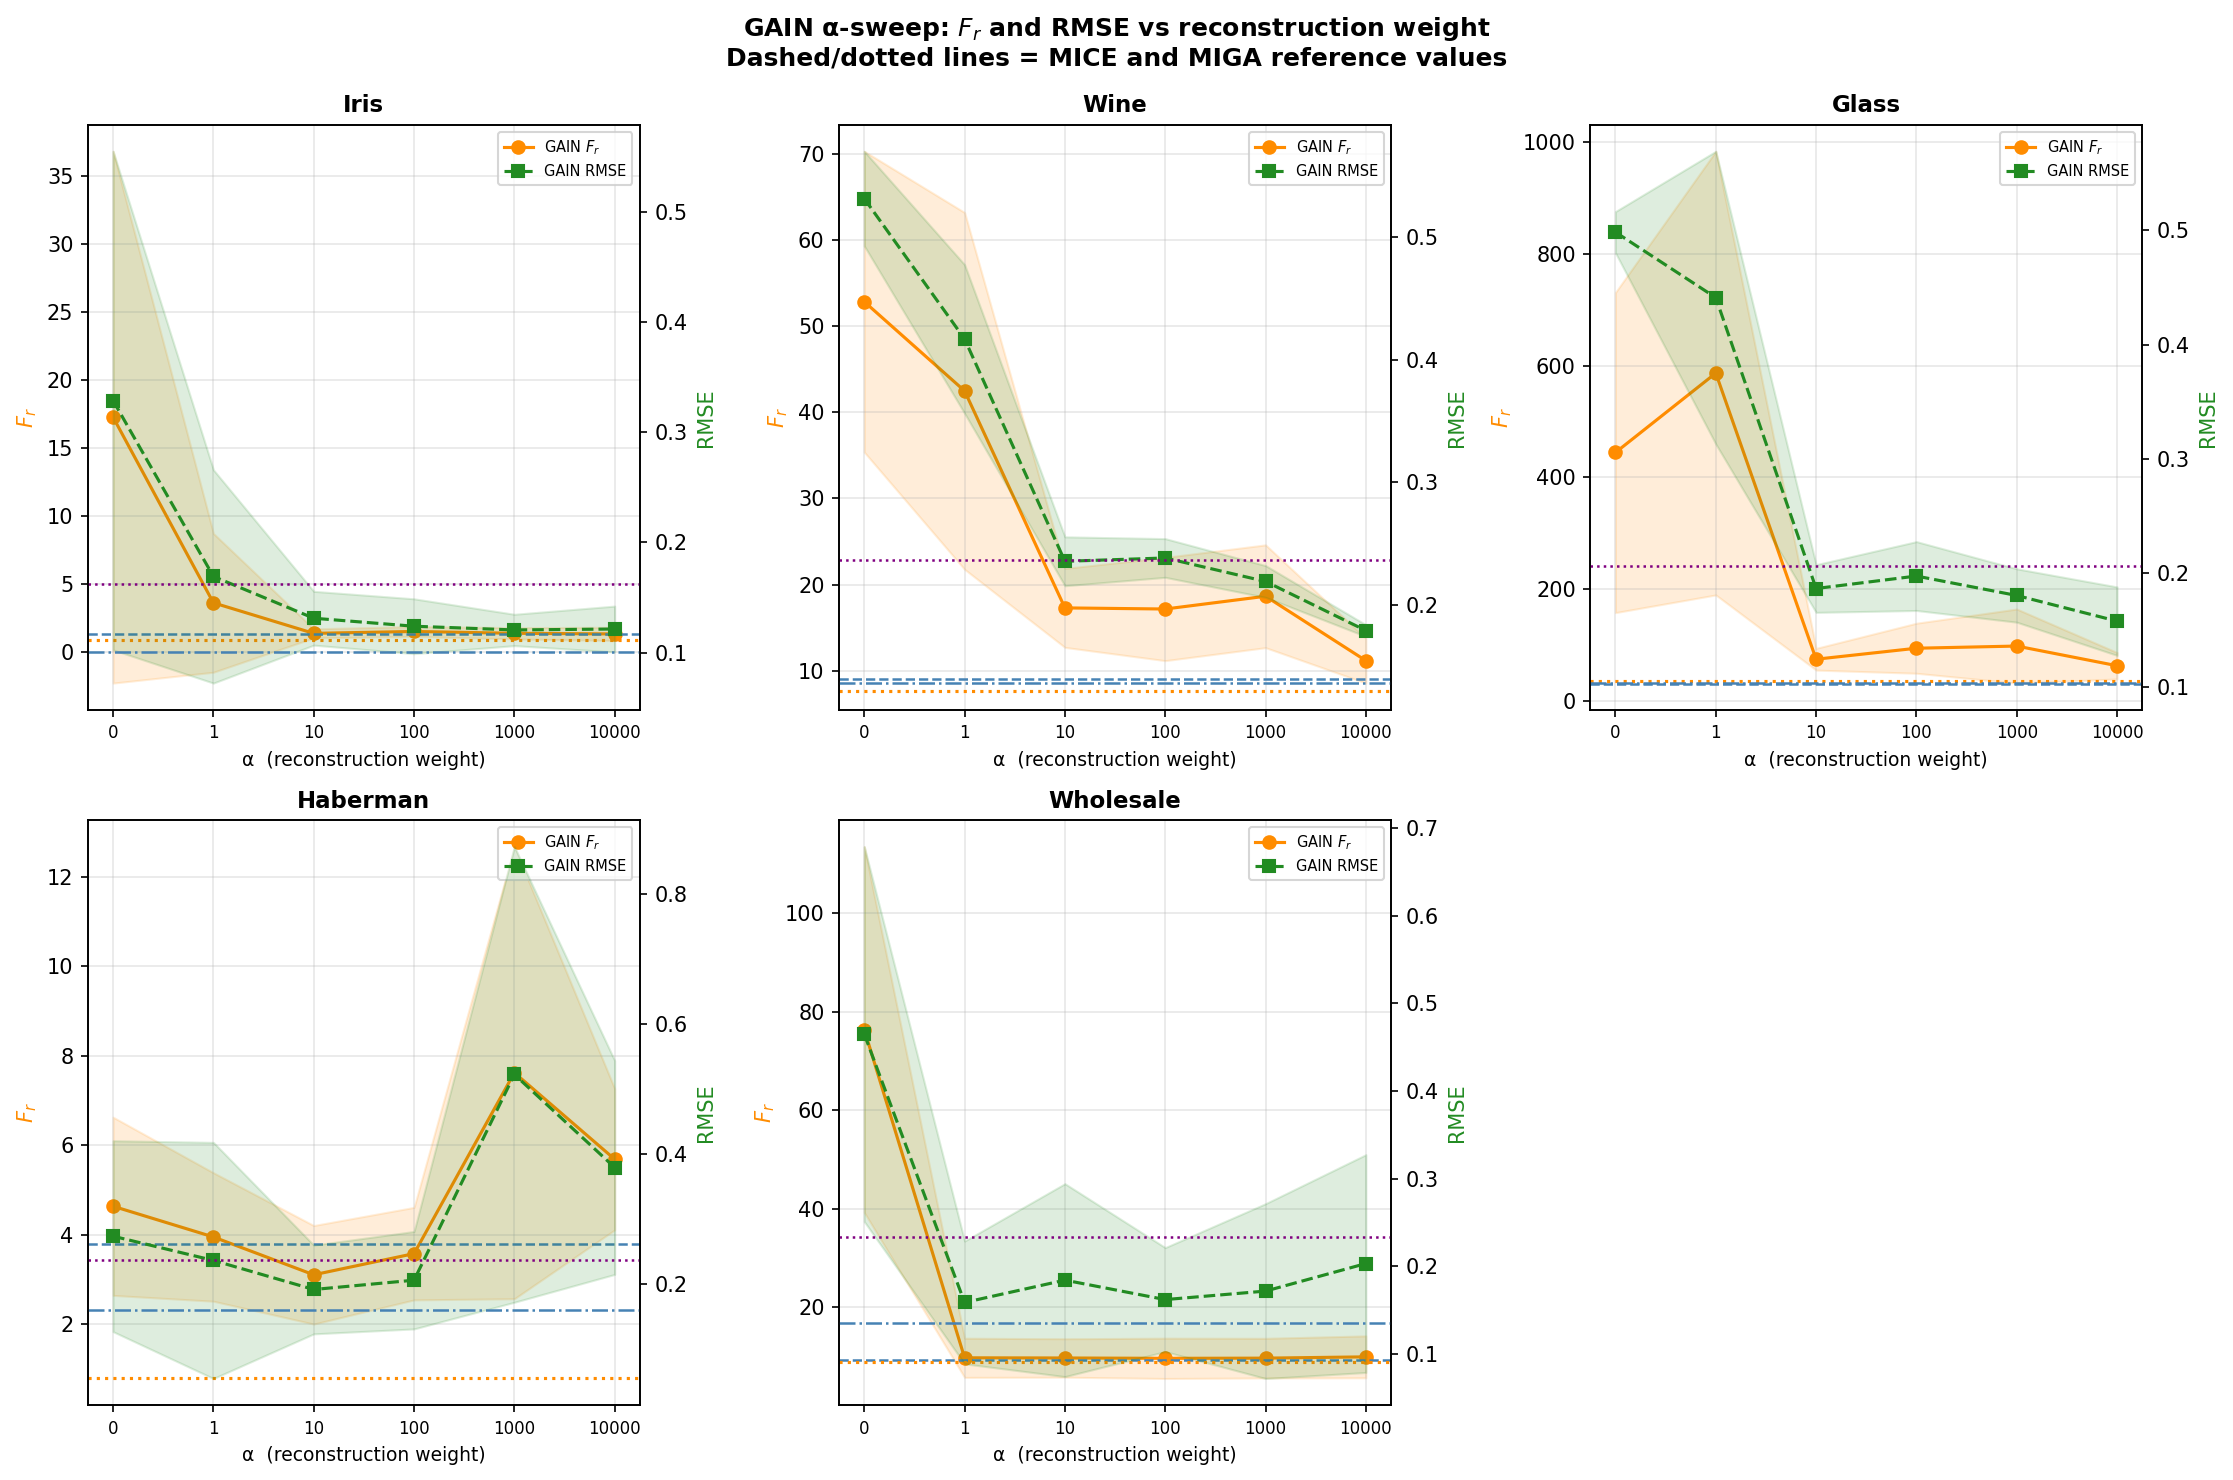
\includegraphics[width=0.85\textwidth]{Figures/fig11_gain_alpha_lines.png}
\caption{$F_r$ and RMSE of GAIN vs $\alpha$. Dashed lines show MICE and MIGA reference values. RMSE never reaches MICE levels at any $\alpha$ on any dataset.}
\label{fig:gain_alpha_lines}
\end{figure}

\textbf{Finding F12 --- No $\alpha$ places GAIN on the Pareto frontier.} The GAIN trajectory lies strictly off the MIGA--MICE frontier across all 5 datasets. On Iris, $\alpha=10$ gives the closest approach ($F_r=1.34$, RMSE$=0.13$) but remains above MICE on both metrics. On Haberman, $\alpha \geq 1000$ causes training instability ($F_r$ spikes to 7.62, RMSE to 0.52). On Glass, every $\alpha$ is dominated by MICE on both metrics. The Fr--RMSE impossibility holds across the full range of reconstruction weights on all 5 datasets.

% Chapter 5 — Discussion (condensed)

\chapter{Discussion}
\label{Chapter5}

\section{The Central Finding}

The most important result of this thesis is that distributional distance ($F_r$) and pointwise accuracy (RMSE) are structurally orthogonal objectives. They do not measure the same underlying quality; optimising one does not optimise the other.

Three lines of evidence establish this. First, under MAR: MIGA achieves significantly lower $F_r$ than MICE on Iris (1.48$\times$, $p=0.001$) and Haberman (1.97$\times$, $p=0.001$), while MICE achieves lower RMSE than MIGA on every dataset (1.4--2.1$\times$). Neither dominates; each wins decisively on its own metric.

Second, the MNAR inversion: on Haberman \texttt{top}, MIGA achieves $F_r = 0.810$ (global minimum) with RMSE = 0.384 (global maximum), and the GA converges to this wrong answer with $\sigma = 0.000005$ across 10 seeds. A method cannot achieve a lower $F_r$ without worsening RMSE more severely.

Third, the formal proof: Propositions~\ref{prop:rmse_implies_fr} and~\ref{prop:fr_implies_rmse} establish that no single imputation can jointly minimise both objectives. The experiments confirm every prediction of the theorem.

Fourth, universality via the GAIN $\alpha$-sweep (C8): Corollary~\ref{cor:gain_orthogonal} proves that GAIN --- which mixes reconstruction and adversarial objectives --- also cannot jointly achieve $F_r=0$ and RMSE$=0$. The empirical $\alpha$-sweep across $\alpha \in \{0, 1, 10, 100, 1000, 10000\}$ on all 5 datasets confirms this: the GAIN arc lies strictly off the MIGA--MICE Pareto frontier at every $\alpha$. On Haberman, high $\alpha$ causes instability; on Glass, every $\alpha$ is dominated by MICE on both metrics. The impossibility holds universally.

\section{When MIGA is the Right Choice}
\label{sec:scope_conditions}

MIGA is appropriate when the downstream analysis requires the correct marginal or joint distribution, not just accurate individual cell values.

\textbf{Confidence intervals and hypothesis tests.} MICE's systematic variance suppression (ratios 0.717--0.976 across datasets) biases within-imputation variance downward, producing overconfident intervals. The downstream evaluation confirms this: MICE's bootstrap 95\% CIs contain the true mean only 10\% of the time on Haberman, versus MIGA's 70\%.

\textbf{Distributional testing.} MICE fails the KS test 100\% of the time on Haberman (by Proposition~\ref{prop:rmse_implies_fr}, this is structurally guaranteed, not dataset-specific). MIGA passes 40\% of the time.

\textbf{Discrete or heavy-tailed features.} MIGA implicitly preserves kurtosis without an explicit kurtosis term: on Haberman, kurtosis distance 1.854 versus MICE's 7.783 (4.2$\times$ better). Matching moments 1--3 incidentally improves moment 4.

\textbf{No cost to predictive accuracy.} All four methods achieve essentially identical classification accuracy ($\approx 0.744$) on Haberman. Choosing MIGA over MICE for distributional tasks is not a trade-off.

MIGA's advantage is reliable when the dataset satisfies two scope conditions: (1) moderate baseline $F_r$ gap --- the distributional distance between $X_A$ and $X_C$ under MAR must be tractable for the GA to close, requiring low-to-moderate dimensionality ($p \lesssim 8$) and low-to-moderate correlation ($\rho \leq 0.6$); and (2) non-degenerate feature variances (no near-zero variance features that inflate the covariance term numerically through $S_A^{-1/2}$). On Glass, the Refractive Index feature ($\sigma^2 \approx 0.00003$) causes seed-to-seed $F_r$ range of 1.6--20.9, making reliable convergence impossible.

\section{When MICE is the Right Choice}

MICE is appropriate when minimum pointwise error is required or when the dataset falls outside MIGA's scope.

\textbf{Predictive modelling.} MICE's 1.4--2.1$\times$ lower RMSE translates directly to better feature quality for downstream regression and classification models.

\textbf{High-dimensional correlated data.} When $p \geq 13$ or $\rho \geq 0.9$, MICE's iterative conditional regression becomes an effective implicit joint distribution estimator. MICE wins both RMSE and $F_r$ on Glass ($p=10$, highly correlated features).

\textbf{Compute constraints.} MIGA requires $\sim$180--210 seconds per seed; MICE runs in under one second. The $Q$ independent runs are embarrassingly parallel ($Q$-fold speedup with no algorithm change), reducing wall-clock time to $\sim$40 seconds, but the per-core cost remains. For large datasets or production pipelines, MICE is more practical.

\section{Relationship to Prior Work}

\subsection{MIGA vs the Original Paper}

Figueroa-Garc\'ia et al.\ (2023) compare MIGA against CMIM and ANNI, both substantially weaker than modern baselines \cite{FigueroaGarcia2023}. Our comparison against MICE and KNN provides the first evaluation of MIGA against current methods. The $F_r$ advantage of MIGA over MICE is confirmed with statistical significance on three of four tested datasets; the RMSE disadvantage is confirmed on all five. The MNAR experiments provide the first characterisation of MIGA's behaviour under non-ignorable missingness, revealing the $F_r \to$ RMSE inversion as a fundamental consequence of the distributional objective under directional selection bias.

\subsection{Relationship to Optimal Transport Imputation}

Muzellec et al.\ (2020) propose imputation via the Sinkhorn divergence \cite{Muzellec2020}. This is conceptually analogous to MIGA's $F_r$ objective: both minimise a measure of distributional discrepancy between the imputed and observed data. Muzellec et al.\ also report that distributional methods achieve higher RMSE than regression-based methods --- an independent empirical confirmation of the $F_r$--RMSE orthogonality theorem. The key algorithmic difference: Sinkhorn divergence is differentiable and enables gradient-based optimisation, but requires $O(n^2 \log n)$ per evaluation; $F_r$ is non-differentiable but evaluable in $O(np^2)$, making it tractable as a GA fitness function over hundreds of thousands of evaluations.

\subsection{Relationship to Proper Multiple Imputation}

Van Buuren (2018, \S3.4) defines ``proper'' imputation as drawing from the full posterior predictive distribution $P(X_{\text{mis}} \mid X_{\text{obs}})$ rather than its conditional mean \cite{vanBuuren2018}. Proper imputation preserves marginal variance by construction. MIGA can be understood as a non-parametric approximation to proper imputation: rather than drawing from a parametric posterior, it uses a GA to find imputations that match distributional moments. MIGA's variance ratios close to 1.0 on Glass (1.005) and Wholesale (1.077) are consistent with the variance-preservation property of proper imputation, and contrast sharply with MICE's systematic under-imputation (ratios 0.717--0.976).

\section{Limitations}

\textbf{MNAR failure mode.} MIGA's fitness function cannot detect that $X_A$ is a biased sample under directional MNAR. The $F_r \to$ RMSE inversion is the most extreme manifestation. IPW-$F_r$ partially corrects this when $n/p \geq 20$, but cannot recover information about values that are entirely absent from the complete-case set.

\textbf{Dimension and correlation interaction.} MIGA fails on Glass ($p=10$) not because $p$ exceeds a threshold in isolation, but because Glass's high inter-feature correlation activates MICE's regression advantage. The $(p, \rho)$ interaction means no simple dimension cutoff applies.

\textbf{Hard dimension limit.} Any dataset with $p \gtrsim 25$ at 30\% MCAR has essentially no complete rows ($n \cdot 0.7^{25} \approx 0.2$ for $n=200$). MIGA cannot operate without a non-trivial $X_A$. This is a fundamental constraint of the distributional reference approach.

\textbf{Single-feature degenerate case.} With only one feature made missing (Haberman, $p=3$), the multivariate covariance term carries little information. The variance over-inflation (ratio 1.535) cannot be corrected without a multivariate constraint.

\section{Future Work}

\textbf{Adaptive diversity injection (AD-MIGA) --- implemented (C7).} Diversity injection fills 90\% of the population with random individuals at every generation. This is fixed regardless of population convergence, wasting budget late in a run when the elite pool has stabilised. AD-MIGA replaces the fixed rate with an exponential decay $\alpha(g) = \exp(-\lambda g/G)$, $\lambda=2.0$, shifting from full exploration at $g=0$ to 13.5\% injection at $g=G$. Results (Section~\ref{sec:ad_miga}) confirm that AD-MIGA achieves lower $F_r$ in fewer convergence generations, while the $F_r$--RMSE orthogonality remains intact.

\textbf{Generalising C2 to neural methods --- Implemented (C8).} Corollary~\ref{cor:gain_orthogonal} extends the impossibility to GAIN, and the $\alpha$-sweep (Section~\ref{sec:gain_alpha_sweep}) confirms it empirically across all 5 datasets and 6 reconstruction weights. The extension to GRAPE \cite{You2020} remains open: its graph-based training mixes reconstruction and structural objectives, suggesting the same impossibility applies, but a formal proof and empirical sweep are needed to complete the universality argument across all neural imputation families.

\textbf{Parallelisation --- Implemented.} The $Q$ independent runs share no state. We add \texttt{n\_jobs} to the MIGA constructor and implement parallel execution via \texttt{concurrent.futures.ProcessPoolExecutor} with \texttt{numpy.random.SeedSequence}-spawned seeds for reproducibility. Benchmarks across all 5 datasets (Q=2, G=200) confirm near-linear scaling: 1.94--1.98$\times$ speedup, consistent across all dimensionalities (Iris 8.7s $\to$ 4.4s, Wine 19.8s $\to$ 10.0s, Glass 19.4s $\to$ 9.8s, Haberman 8.9s $\to$ 4.6s, Wholesale 28.6s $\to$ 14.5s). At Q=6, wall-clock time reduces from $\sim$200s to $\sim$35s per seed.

\textbf{Moment expansion.} Adding a kurtosis term $D_r(k_A, k_C)$ to $F_r$ could widen MIGA's already-observed kurtosis advantage. A longer-term alternative is replacing the three-moment $F_r$ with MMD or Wasserstein distance for a complete distributional comparison.

\section{Summary}

This thesis established six contributions:

\begin{enumerate}
    \item \textbf{MIGA can be faithfully reimplemented} (C1). The open-source Python implementation achieves paper-level results on five benchmark datasets.

    \item \textbf{The $F_r$--RMSE orthogonality is formally provable and empirically confirmed} (C2). Propositions~\ref{prop:rmse_implies_fr}--\ref{prop:fr_implies_rmse} prove that no single imputation can jointly minimise both objectives. Every experiment confirms this: MIGA wins $F_r$ where it is competitive; MICE wins RMSE without exception.

    \item \textbf{MIGA fails under directional MNAR in a characterisable and correctable way} (C3, C6). The $F_r \to$ RMSE inversion is the sharpest empirical confirmation of C2. IPW-$F_r$ partially corrects this when $n/p \geq 20$, reducing $F_r$ by up to 38\%.

    \item \textbf{MIGA's $F_r$ advantage is real but bounded} (C4). MIGA wins $F_r$ on Iris, Haberman, and Wholesale ($p \leq 8$) with statistical significance. MICE wins RMSE on all five datasets.

    \item \textbf{The failure mode depends jointly on $(p, \rho)$, not dimension alone} (C5). MIGA wins for $p \leq 13$ at $\rho \leq 0.6$; loses at $\rho = 0.9$ even for $p = 8$.

    \item \textbf{MIGA's distributional advantage propagates to downstream utility under well-conditioned scope conditions.} On Haberman, MIGA is the only method to pass the KS test (40\% vs 0\%) and achieves 70\% CI coverage versus MICE's 10\%, at zero cost to classification accuracy.

    \item \textbf{AD-MIGA achieves lower $F_r$ in fewer generations (C7).} Replacing the fixed 90\% diversity injection with exponential decay $\alpha(g) = \exp(-\lambda g/G)$ reduces convergence generation without degrading RMSE. The $F_r$--RMSE orthogonality is preserved across all three tested datasets.

    \item \textbf{The $F_r$--RMSE impossibility is universal across neural methods (C8).} Corollary~\ref{cor:gain_orthogonal} extends C2 to GAIN. The empirical $\alpha$-sweep across 6 reconstruction weights and all 5 datasets confirms three failure regimes: monotone-but-off-frontier (Iris, Wine), training instability at high $\alpha$ (Haberman), and total MICE-domination (Glass). The impossibility holds universally across all $\alpha$ and all datasets.

    \item \textbf{Parallel execution reduces wall-clock time by $Q\times$.} The \texttt{n\_jobs} parameter parallelises the $Q$ independent runs via \texttt{ProcessPoolExecutor}. Benchmarks on all 5 datasets confirm near-linear scaling (1.94--1.98$\times$ at Q=2). At Q=6, runtime falls from $\sim$200s to $\sim$35s per seed.
\end{enumerate}

The recommendation: use MIGA when the downstream analysis requires the correct distribution \emph{and} $p \lesssim 8$, $\rho \lesssim 0.6$, and feature variances are well-conditioned. Use MICE when minimum pointwise error or compute efficiency is required. No neural method mixing reconstruction and adversarial objectives provides a free lunch between the two extremes.


\end{spacing}

\printbibliography[heading=bibintoc]

\end{sloppypar}
\end{document}
